\documentclass[11pt,a4paper]{article}

\usepackage[utf8]{inputenc}
\usepackage[T1]{fontenc}
\usepackage{lmodern}
\usepackage[english]{babel}
\usepackage{geometry}
\usepackage{graphicx}
\usepackage{float}
\usepackage{caption}
\usepackage{amsmath}
\usepackage{booktabs}
\usepackage{hyperref}
\usepackage{subcaption}

\geometry{margin=1in}

% Leave pages "short" when content does not fill them, rather than spreading
% the text down to the bottom. Avoids ghost gaps when an [H] figure does not
% fit on the current page and is pushed onto the next one.
\raggedbottom

\title{Empirical Analysis of Transformers on Graph Connectivity}
\author{Edoardo Paccagnella}
\date{\today}

\begin{document}

\maketitle

\section{Introduction}
\label{sec:intro}

This report is a working summary of a sequence of experiments on a
transformer trained to predict the connectivity matrix of an input graph. The
starting point is the paper
\emph{Transformers Provably Learn Algorithmic Solutions for Graph
Connectivity, But Only with the Right Data} (Ye, Fu, Jia, Sharan, 2026), which
proves that for the simplified \emph{Disentangled Transformer} architecture an
$L$\nobreakdash-layer model can solve connectivity on graphs of diameter at
most $3^L$, and that training the model exclusively on within-capacity
graphs (the \emph{data lever}) provably drives the model towards the
algorithmic, matrix-powering solution rather than a degree-based heuristic.
The motivating question of this report is whether the same data lever
empirically helps a \emph{standard} (non-disentangled) transformer in the
same setting.

The experiments were run in the following order, and each step was decided as
a reaction to what the previous step showed.

\begin{enumerate}
    \item \textbf{Small-scale in-distribution checks
    (Chapter~\ref{sec:ch1}).} We first trained the standard transformer
    on Erd\H{o}s--R\'enyi graphs with $n = 10$ and on the two structured
    families (2-chains and 2-cliques) at $n = 14$ used in the paper. The goal
    was only to verify that the model and the training pipeline behave
    reasonably in distribution and to get a baseline OOD picture. We
    deliberately do not draw strong conclusions from these experiments: the
    graphs are small and the in-distribution accuracy is essentially
    saturated, so the regime is not informative about the algorithm versus
    heuristic question.

    \item \textbf{Diameter-controlled training on
    ER$(n = 40, p = 0.05)$ with the small model (Chapter~\ref{sec:ch2}).}
    We then moved to the setting that is actually relevant to the data
    lever: $n = 40$, $p = 0.05$, so that the three diameter cutoffs of
    interest $D \le 7$, $D \le 9$, $D \le 11$ accept genuinely different
    fractions of graphs ($\sim 14\%, 55\%, 84\%$) and are statistically
    distinguishable. We trained four parallel runs (unfiltered, $D \le 11$,
    $D \le 9$, $D \le 7$), kept the model architecture identical
    ($d_{\mathrm{model}} = 64$, 1 head, 2 layers), and compared
    convergence speed, in-distribution accuracy, and OOD behaviour on
    2-chains, 2-cliques, and unfiltered ER (broken down by graph diameter).
    The four small-model runs all settle at the same exact-match
    accuracy of about $0.80$, which strongly suggested a model-capacity
    bottleneck rather than a data-distribution effect.

    \item \textbf{Same diameter-controlled experiments with a larger model
    (Chapter~\ref{sec:ch3}).} To check the capacity hypothesis we re-ran the
    four diameter-controlled training experiments with a larger model
    ($d_{\mathrm{model}} = 512$, $d_{\mathrm{ff}} = 2048$, $\sim 6.3$M
    parameters), an online streaming data pipeline (so the model never sees
    the same graph twice), bf16 mixed precision, normalised-ReLU attention
    in place of softmax, and a $1{,}000{,}000$-step training budget. We
    also added a 4-phase curriculum
    ($D \le 7 \to D \le 9 \to D \le 10 \to D \le 11$). With this model the
    in-distribution ceiling lifts and every run reaches
    $\ge 99.95\%$ exact match. We then re-evaluated all five trained models
    on the same OOD benchmark as Chapter~\ref{sec:ch2}.
\end{enumerate}

Throughout the report we describe what we observe and try to avoid
overinterpreting it. The data lever proposed by the paper turns out to be
\emph{useful for convergence speed} but, in our standard-transformer setup,
\emph{not useful for OOD generalisation}: across all the OOD tests we ran,
the unfiltered model is at least as good as any of the diameter-restricted
specialists, and on the harder OOD distributions (chains at large
$n_{\text{active}}$, 2-cliques) all five large-model variants fail in
qualitatively the same way. This is the main empirical finding of the
report.

\section{Model and task}
\label{sec:model}

We use a \emph{Graph Connectivity Transformer} trained to predict the full
connectivity matrix of an input graph.

Given an undirected graph with $n$ nodes (the value of $n$ varies across
experiments and is specified in each chapter), the input is its adjacency
matrix with self-loops added,
\[
A \in \{0,1\}^{n \times n}.
\]
The target is the connectivity matrix
\[
R \in \{0,1\}^{n \times n}, \qquad
R_{ij} = 1 \iff i \text{ and } j \text{ belong to the same connected component.}
\]

Two model configurations are used across the report.

\paragraph{Small configuration} (Chapters~\ref{sec:ch1} and~\ref{sec:ch2}):
\begin{itemize}
    \item Layers: 2, attention heads: 1, $d_{\mathrm{model}} = 64$,
          $d_{\mathrm{ff}} = 128$.
    \item Softmax attention, no dropout, batch size $256$.
    \item Optimiser: AdamW, learning rate $10^{-3}$, weight decay $10^{-2}$,
          gradient clipping $1.0$.
    \item Training steps: $500{,}000$, evaluation every $1{,}000$ steps.
    \item Fixed pre-generated training set of $6{,}000{,}000$ graphs, fixed
          test set of $10{,}000$ graphs.
    \item Parameter count: $\sim 72$k.
\end{itemize}

\paragraph{Large configuration} (Chapter~\ref{sec:ch3}):
\begin{itemize}
    \item Layers: 2, attention heads: 4, $d_{\mathrm{model}} = 512$,
          $d_{\mathrm{ff}} = 2048$.
    \item Normalised-ReLU attention ($\alpha = \tfrac{1}{n}\,\mathrm{ReLU}(QK^\top/\sqrt{d_h})$),
          no dropout, batch size $1{,}000$.
    \item Optimiser: AdamW, peak learning rate $10^{-4}$ with linear
          warm-up and cosine decay, weight decay $10^{-4}$, gradient
          clipping $1.0$, bf16 mixed precision.
    \item Training steps: $1{,}000{,}000$, evaluation every $5{,}000$
          steps on a pre-generated test set of $10{,}000$ graphs.
    \item Training data is generated \emph{on the fly} via rejection
          sampling: the model never sees the same training graph twice
          (effective training set size $\approx 10^9$ graphs).
    \item Parameter count: $6{,}347{,}304$.
\end{itemize}

In every experiment we track the following metrics on the held-out test set:
\begin{itemize}
    \item \textbf{Exact-match accuracy:} fraction of test graphs for which
          the predicted connectivity matrix is exactly correct.
    \item \textbf{Pairwise accuracy:} average accuracy across all ordered
          node pairs in the test set.
    \item \textbf{Pairwise accuracy by distance:} pairwise accuracy
          conditioned on the shortest-path distance between the two nodes
          in the test graph.
    \item \textbf{Training loss:} binary cross-entropy loss.
\end{itemize}

\vspace{1em}

\section{Chapter 1 --- Small-scale experiments ($n = 10$ and $n = 14$)}
\label{sec:ch1}

The purpose of this chapter is to document the warm-up experiments. The model
is the small configuration of Section~\ref{sec:model}, with the training
sets and graph sizes specified in each subsection. As argued in the
introduction, these experiments are not designed to discriminate between an
algorithmic and a heuristic solution: the graphs are small, the in-distribution
accuracy saturates very quickly, and the only OOD test set we use here
(ER$(n = 14)$ at three densities) is a structurally simple shift. We
therefore restrict the discussion to a brief description of each run and a
short note on what the figures show.

\subsection{ER$(n = 10)$}

\begin{figure}[H]
    \centering
    \begin{subfigure}[t]{0.48\textwidth}
        \centering
        
\includegraphics[width=\textwidth]{runs/retrain_er_3352759/n10_p0.2_rep0/retrain_er_p02_accuracy.png}
        \caption{Exact match and pairwise accuracy ($p = 0.2$).}
    \end{subfigure}
    \hfill
    \begin{subfigure}[t]{0.48\textwidth}
        \centering
        
\includegraphics[width=\textwidth]{runs/retrain_er_3352759/n10_p0.2_rep0/retrain_er_p02_train_loss.png}
        \caption{Training loss ($p = 0.2$).}
    \end{subfigure}

    \vspace{1em}

    \begin{subfigure}[t]{0.8\textwidth}
        \centering
        
\includegraphics[width=\textwidth]{runs/retrain_er_3352759/n10_p0.2_rep0/per_distance_accuracy_small_multiples_p02.png}
        \caption{Pairwise accuracy by shortest-path distance ($p = 0.2$). The number above each panel is the count of test pairs at that distance.}
    \end{subfigure}

    \caption{ER$(n = 10,\, p = 0.2)$ training run.}
\end{figure}

\begin{figure}[H]
    \centering
    \begin{subfigure}[t]{0.48\textwidth}
        \centering
        
\includegraphics[width=\textwidth]{runs/retrain_er_3352759/n10_p0.5_rep0/retrain_er_p05_accuracy.png}
        \caption{Exact match and pairwise accuracy ($p = 0.5$).}
    \end{subfigure}
    \hfill
    \begin{subfigure}[t]{0.48\textwidth}
        \centering
        
\includegraphics[width=\textwidth]{runs/retrain_er_3352759/n10_p0.5_rep0/retrain_er_p05_train_loss.png}
        \caption{Training loss ($p = 0.5$).}
    \end{subfigure}

    \vspace{1em}

    \begin{subfigure}[t]{0.8\textwidth}
        \centering
        
\includegraphics[width=\textwidth]{runs/retrain_er_3352759/n10_p0.5_rep0/per_distance_accuracy_small_multiples_p05.png}
        \caption{Pairwise accuracy by shortest-path distance ($p = 0.5$). The number above each panel is the count of test pairs at that distance.}
    \end{subfigure}

    \caption{ER$(n = 10,\, p = 0.5)$ training run.}
\end{figure}

\paragraph{What the figures show.} Both runs saturate within the first few
thousand steps. The loss curves are very small but show a slight residual
oscillation. Per-distance accuracy is essentially perfect up to the largest
distance reasonably represented in the test set; the few visible drops at
$d \ge 6$ are on bins that contain very few samples.

\subsection{2-chains ($n = 14$)}

\begin{figure}[H]
    \centering
    \begin{subfigure}[t]{0.48\textwidth}
        \centering
        
\includegraphics[width=\textwidth]{runs/retrain_2chains_3352759/n14_k7_rep0/retrain_two_chains_k07_accuracy.png}
        \caption{Exact match and pairwise accuracy.}
    \end{subfigure}
    \hfill
    \begin{subfigure}[t]{0.48\textwidth}
        \centering
        
\includegraphics[width=\textwidth]{runs/retrain_2chains_3352759/n14_k7_rep0/retrain_two_chains_k07_train_loss.png}
        \caption{Training loss.}
    \end{subfigure}

    \vspace{1em}

    \begin{subfigure}[t]{0.8\textwidth}
        \centering
        
\includegraphics[width=\textwidth]{runs/retrain_2chains_3352759/n14_k7_rep0/per_distance_accuracy_small_multiples_k07.png}
        \caption{Pairwise accuracy by shortest-path distance. The number above each panel is the count of test pairs at that distance.}
    \end{subfigure}

    \caption{2-chains $(n = 14, k = 7)$ training run.}
\end{figure}

\paragraph{What the figures show.} The model reaches near-perfect accuracy
very quickly. The training loss exhibits a clear periodic spike pattern
which we discuss next.

\subsubsection{Periodic spikes in the training loss}
\label{sec:loss-spikes}

The training-loss curve shows periodic spikes of magnitude
$\sim 0.01$--$0.015$, appearing roughly every $25{,}000$--$30{,}000$ steps.
The period matches the epoch length: with $6{,}000{,}000$ training graphs
and batch size $256$, one epoch is
\[
T_{\mathrm{epoch}}
= \frac{6{,}000{,}000}{256} \approx 23{,}438
\]
training steps. At each epoch boundary the dataset is reshuffled. Because
AdamW maintains running estimates of the first and second moments of the
gradients calibrated on the previous local sequence of minibatches, the
sudden change in mini-batch order produces a short transient mismatch
between the optimiser state and the new local gradient statistics; after
a few hundred steps the optimiser re-adapts and the loss returns to its
baseline. The observed period is slightly longer than $T_{\mathrm{epoch}}$
because the displayed loss is a $1{,}000$-step moving average.

\subsubsection{Out-of-distribution evaluation (chains $\to$ ER)}

\begin{figure}[H]
    \centering
    
\includegraphics[width=\textwidth]{runs/ood_cross_experiment/ood_2chains_per_distance_bars.png}
    \caption{2-chains $(n = 14)$ model evaluated on ER$(n = 14, p)$ for
    $p \in \{0.05, 0.2, 0.5\}$. Per-distance pairwise accuracy.}
\end{figure}

Exact-match accuracy is $\approx 0$ at all three densities and pairwise
accuracy lies in $0.50$--$0.52$. The per-distance breakdown shows that
accuracy is highest at $d = 1, 2$ and decays for larger distances; the
``disconnected'' bin is the largest source of error.

\subsection{2-cliques ($n = 14$)}

\begin{figure}[H]
    \centering
    \begin{subfigure}[t]{0.48\textwidth}
        \centering
        
\includegraphics[width=\textwidth]{runs/retrain_2cliques_3352759/n14_k7_rep0/retrain_two_cliques_k07_accuracy.png}
        \caption{Exact match and pairwise accuracy.}
    \end{subfigure}
    \hfill
    \begin{subfigure}[t]{0.48\textwidth}
        \centering
        
\includegraphics[width=\textwidth]{runs/retrain_2cliques_3352759/n14_k7_rep0/retrain_two_cliques_k07_train_loss.png}
        \caption{Training loss.}
    \end{subfigure}

    \vspace{1em}

    \begin{subfigure}[t]{0.8\textwidth}
        \centering
        
\includegraphics[width=\textwidth]{runs/retrain_2cliques_3352759/n14_k7_rep0/per_distance_accuracy_small_multiples_k07.png}
        \caption{Pairwise accuracy by shortest-path distance. The number above each panel is the count of test pairs at that distance.}
    \end{subfigure}

    \caption{2-cliques $(n = 14, k = 7)$ training run.}
\end{figure}

\paragraph{What the figures show.} The 2-cliques family with $n = 14$ and
$k = 7$ has only $\binom{14}{7}/2 = 1716$ distinct graphs; we therefore use
the exhaustive set split $80\%/20\%$ and cap training at $800$ steps. The
model saturates within a few hundred steps; in-distribution accuracy on
this dataset is mainly evidence of memorisation rather than of generalisation.

\subsubsection{Out-of-distribution evaluation (cliques $\to$ ER)}

\begin{figure}[H]
    \centering
    
\includegraphics[width=\textwidth]{runs/ood_cross_experiment/ood_2cliques_per_distance_bars.png}
    \caption{2-cliques $(n = 14, k = 7)$ model evaluated on ER$(n = 14, p)$
    for $p \in \{0.05, 0.2, 0.5\}$. Per-distance pairwise accuracy.}
\end{figure}

Exact match is $0\%$ at all three densities. The per-distance breakdown is
informative: the model gets $d = 1$ pairs essentially right
(${\ge}0.99$ at $p = 0.2, 0.5$ and $1.000$ at $p = 0.05$) and collapses to
near-zero accuracy for $d \ge 2$. Effectively the trained model has learnt
the rule
\[
\hat{R}_{ij} = 1 \iff \text{$i$ and $j$ share a direct edge in $A$,}
\]
which is the correct answer inside a clique but not on a generic graph.

\vspace{2em}

\section{Chapter 2 --- Diameter-controlled training on ER$(n = 40)$ (small model)}
\label{sec:ch2}

\subsection{Motivation and setup}

The small-scale experiments of Chapter~\ref{sec:ch1} are not informative
about the question we ultimately care about, namely whether the
\emph{data lever} of the disentangled-transformer paper transfers to a
standard transformer. To probe that question we need a regime in which (i)
the model has to do non-trivial multi-hop reasoning, (ii) the diameter
cut-offs $D \le 7$, $D \le 9$, $D \le 11$ produce \emph{visibly different}
training distributions, and (iii) the model is still small enough that we
can train four parallel runs to convergence.

The choice $n = 40$, $p = 0.05$ (expected degree $np = 2$) makes the
diameter cut-offs statistically meaningful: at this density the three
cut-offs accept respectively $\approx 14\%$, $55\%$, and $84\%$ of randomly
sampled graphs. With smaller $n$ (e.g.\ $n = 20$) all three cut-offs accept
more than $95\%$ of graphs and the comparison becomes degenerate.

We run four parallel experiments with the small configuration of
Section~\ref{sec:model}, identical except for the diameter filter applied
to the training graphs:
\begin{itemize}
    \item \textbf{Unfiltered:} ER$(40, 0.05)$.
    \item \textbf{$D \le 11$:} ER$(40, 0.05)$ rejecting any graph whose
          largest finite shortest-path distance exceeds $11$.
    \item \textbf{$D \le 9$:} same with cut-off $9$. This is the
          \emph{predicted optimum} for a $2$-layer model, since $3^L = 9$.
    \item \textbf{$D \le 7$:} same with cut-off $7$.
\end{itemize}
Each run uses $6{,}000{,}000$ training graphs, $10{,}000$ in-distribution
test graphs (drawn from the same filtered distribution), and $500{,}000$
optimisation steps.

\subsection{Cross-experiment view: convergence and final accuracy}
\label{sec:ch2-cross-in}

Table~\ref{tab:n40-summary} summarises the four runs. The most striking
effect is on convergence speed: tighter diameter constraints lead to
much faster learning, with the most restrictive cut-off ($D \le 7$)
roughly $17\times$ faster than the unfiltered run on the
``$99\%$-pairwise-accuracy'' milestone.

\begin{table}[H]
\centering
\begin{tabular}{lcccc}
\toprule
Experiment & Best exact match & Final pairwise & Final loss & Steps to $99\%$ pairwise \\
\midrule
Unfiltered   & 0.812 & 0.990 & 0.0260 & $273{,}000$ \\
$D \le 11$   & 0.808 & 0.993 & 0.0193 & $\phantom{0}78{,}000$ \\
$D \le 9$    & 0.802 & 0.995 & 0.0135 & $\phantom{0}38{,}000$ \\
$D \le 7$    & \textbf{0.823} & 0.998 & 0.0060 & $\phantom{0}\textbf{16{,}000}$ \\
\bottomrule
\end{tabular}
\caption{Summary of the four diameter-controlled small-model experiments
on ER$(n = 40, p = 0.05)$. All runs use $6{,}000{,}000$ training graphs
and $500{,}000$ optimisation steps.}
\label{tab:n40-summary}
\end{table}

\begin{figure}[H]
    \centering
    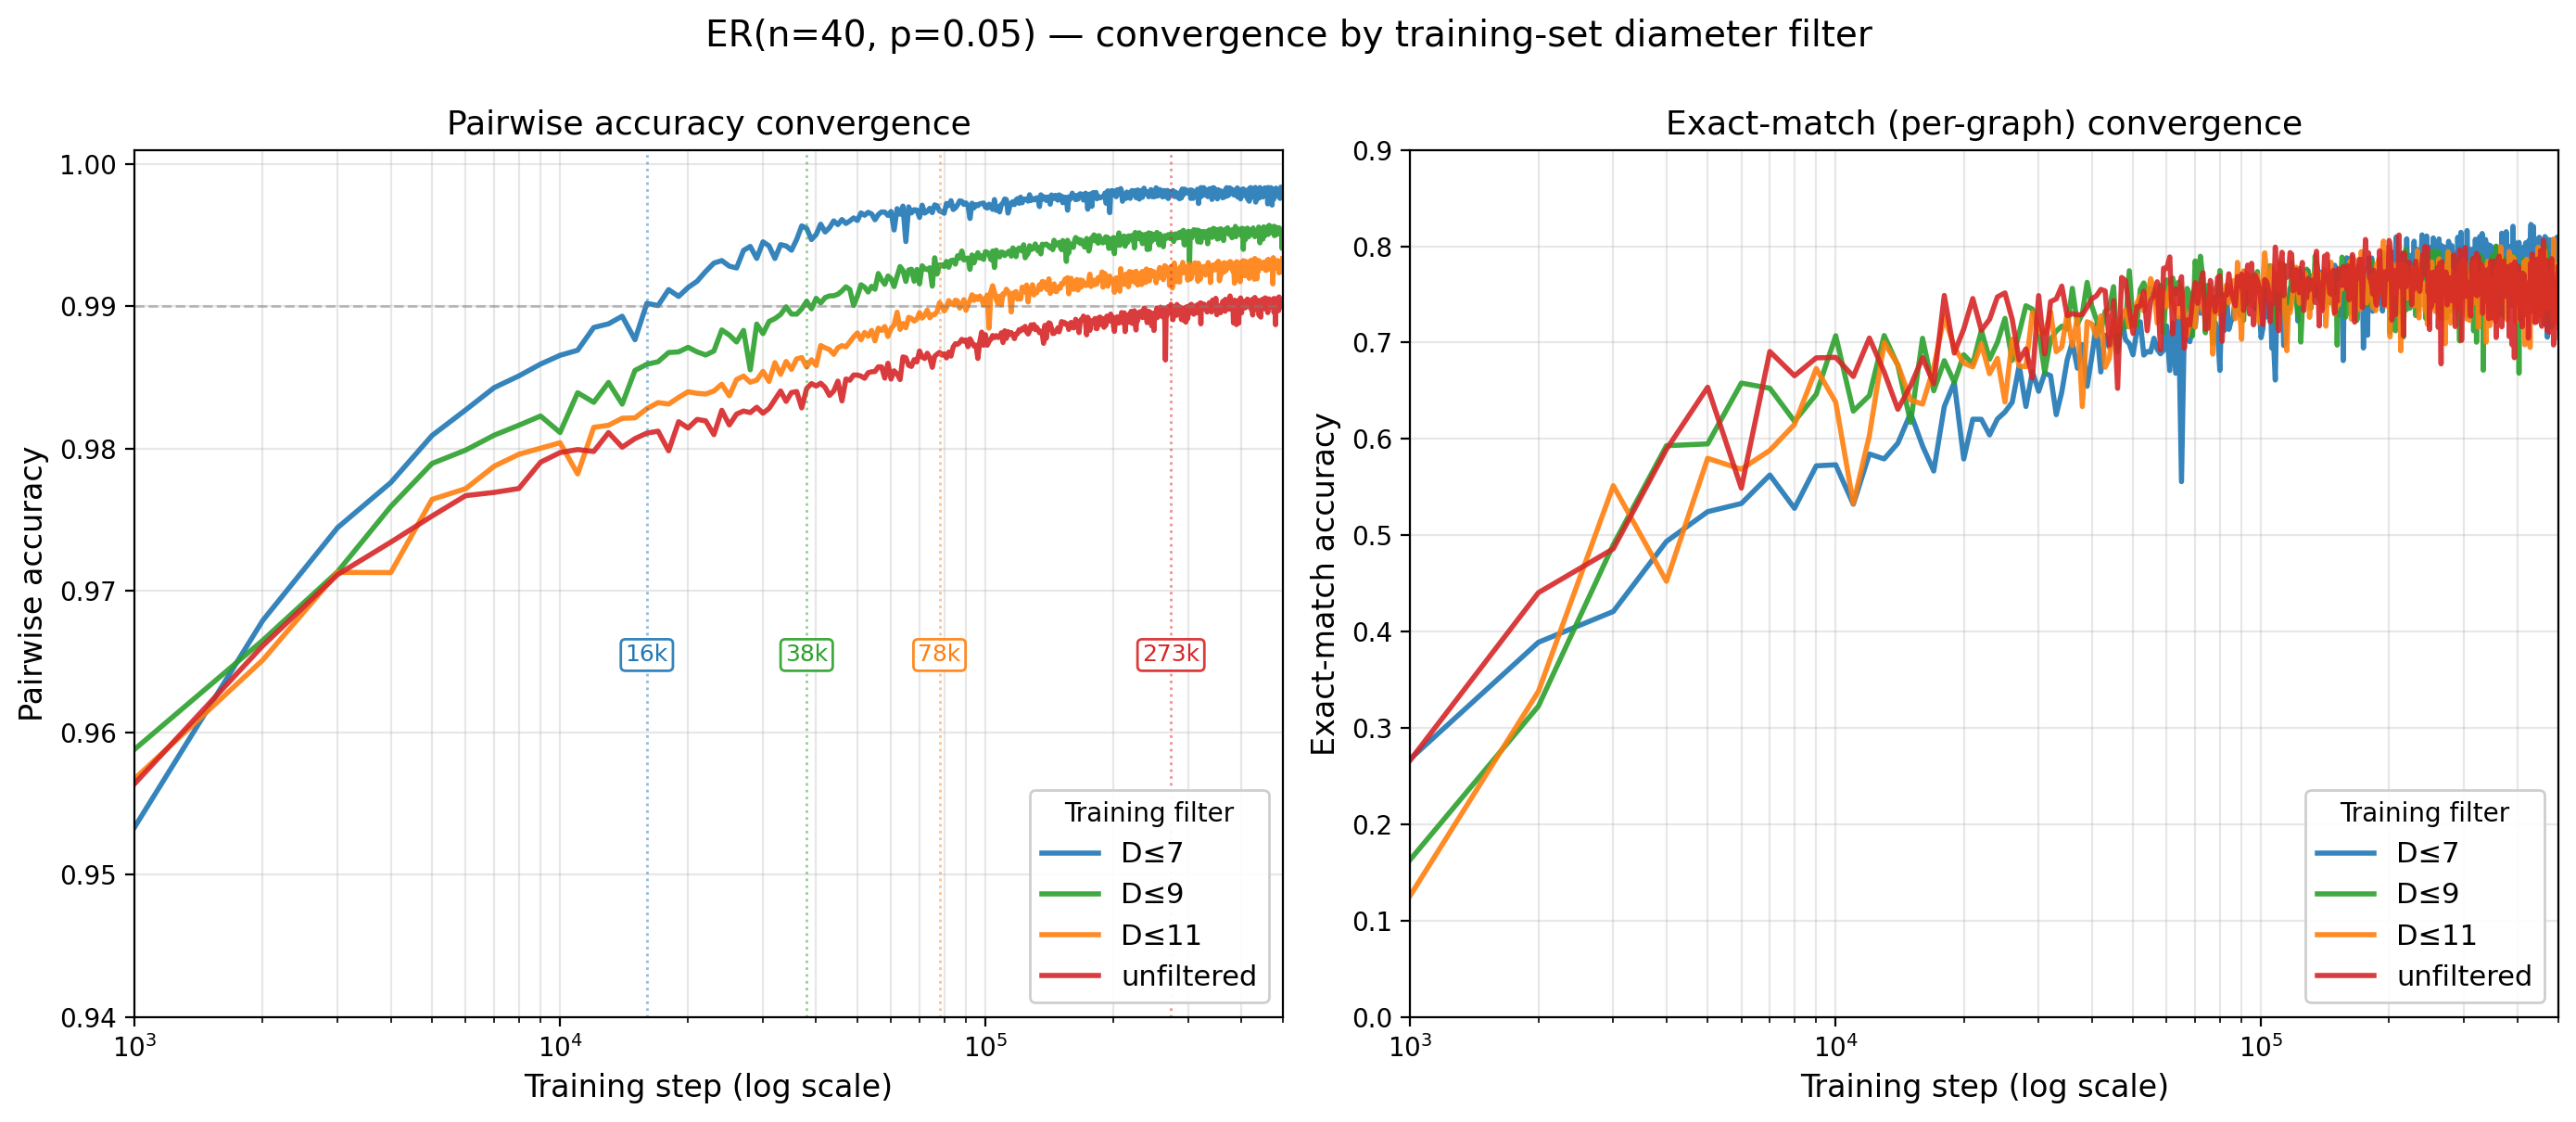
\includegraphics[width=\textwidth]{runs/n40_cross_experiment/01_convergence.png}
    \caption{Convergence comparison across the four diameter-controlled
    experiments. \emph{Left:} pairwise accuracy as a function of the
    training step (log scale); boxed labels mark the step at which each
    model first crosses the $99\%$ threshold (dashed line).
    \emph{Right:} per-graph exact-match accuracy on the same log-scaled
    axis. Despite the large gap in convergence speed, all four runs
    settle at very similar final values.}
    \label{fig:n40-convergence}
\end{figure}

\paragraph{Convergence speed is monotone in the diameter filter.} Tighter
constraints lead to faster learning. This is consistent with the picture
proposed by the disentangled-transformer paper, in which an $L$-layer
model is expected to learn most efficiently on graphs whose diameter does
not exceed $3^L$.

\paragraph{Final accuracy is essentially unaffected.} All four runs
settle in a narrow band around $80\%$ exact match and $99\%$ pairwise
accuracy. With $n = 40$ each test graph contains $40 \times 39 = 1{,}560$
off-diagonal pairs, so a pairwise accuracy of $0.99$ corresponds on
average to about $15$ wrong pairs per graph, which is enough to drive the
exact-match metric down. The fact that all four runs land at roughly
$0.80$ exact match strongly suggests that the bottleneck of the present
setup is the size of the model ($d_{\mathrm{model}} = 64$, one head, two
layers) rather than the structure of the training data; this is the
direct motivation for the large-model experiments of
Chapter~\ref{sec:ch3}.

\subsection{Cross-experiment view: pairwise accuracy by distance}

\begin{figure}[H]
    \centering
    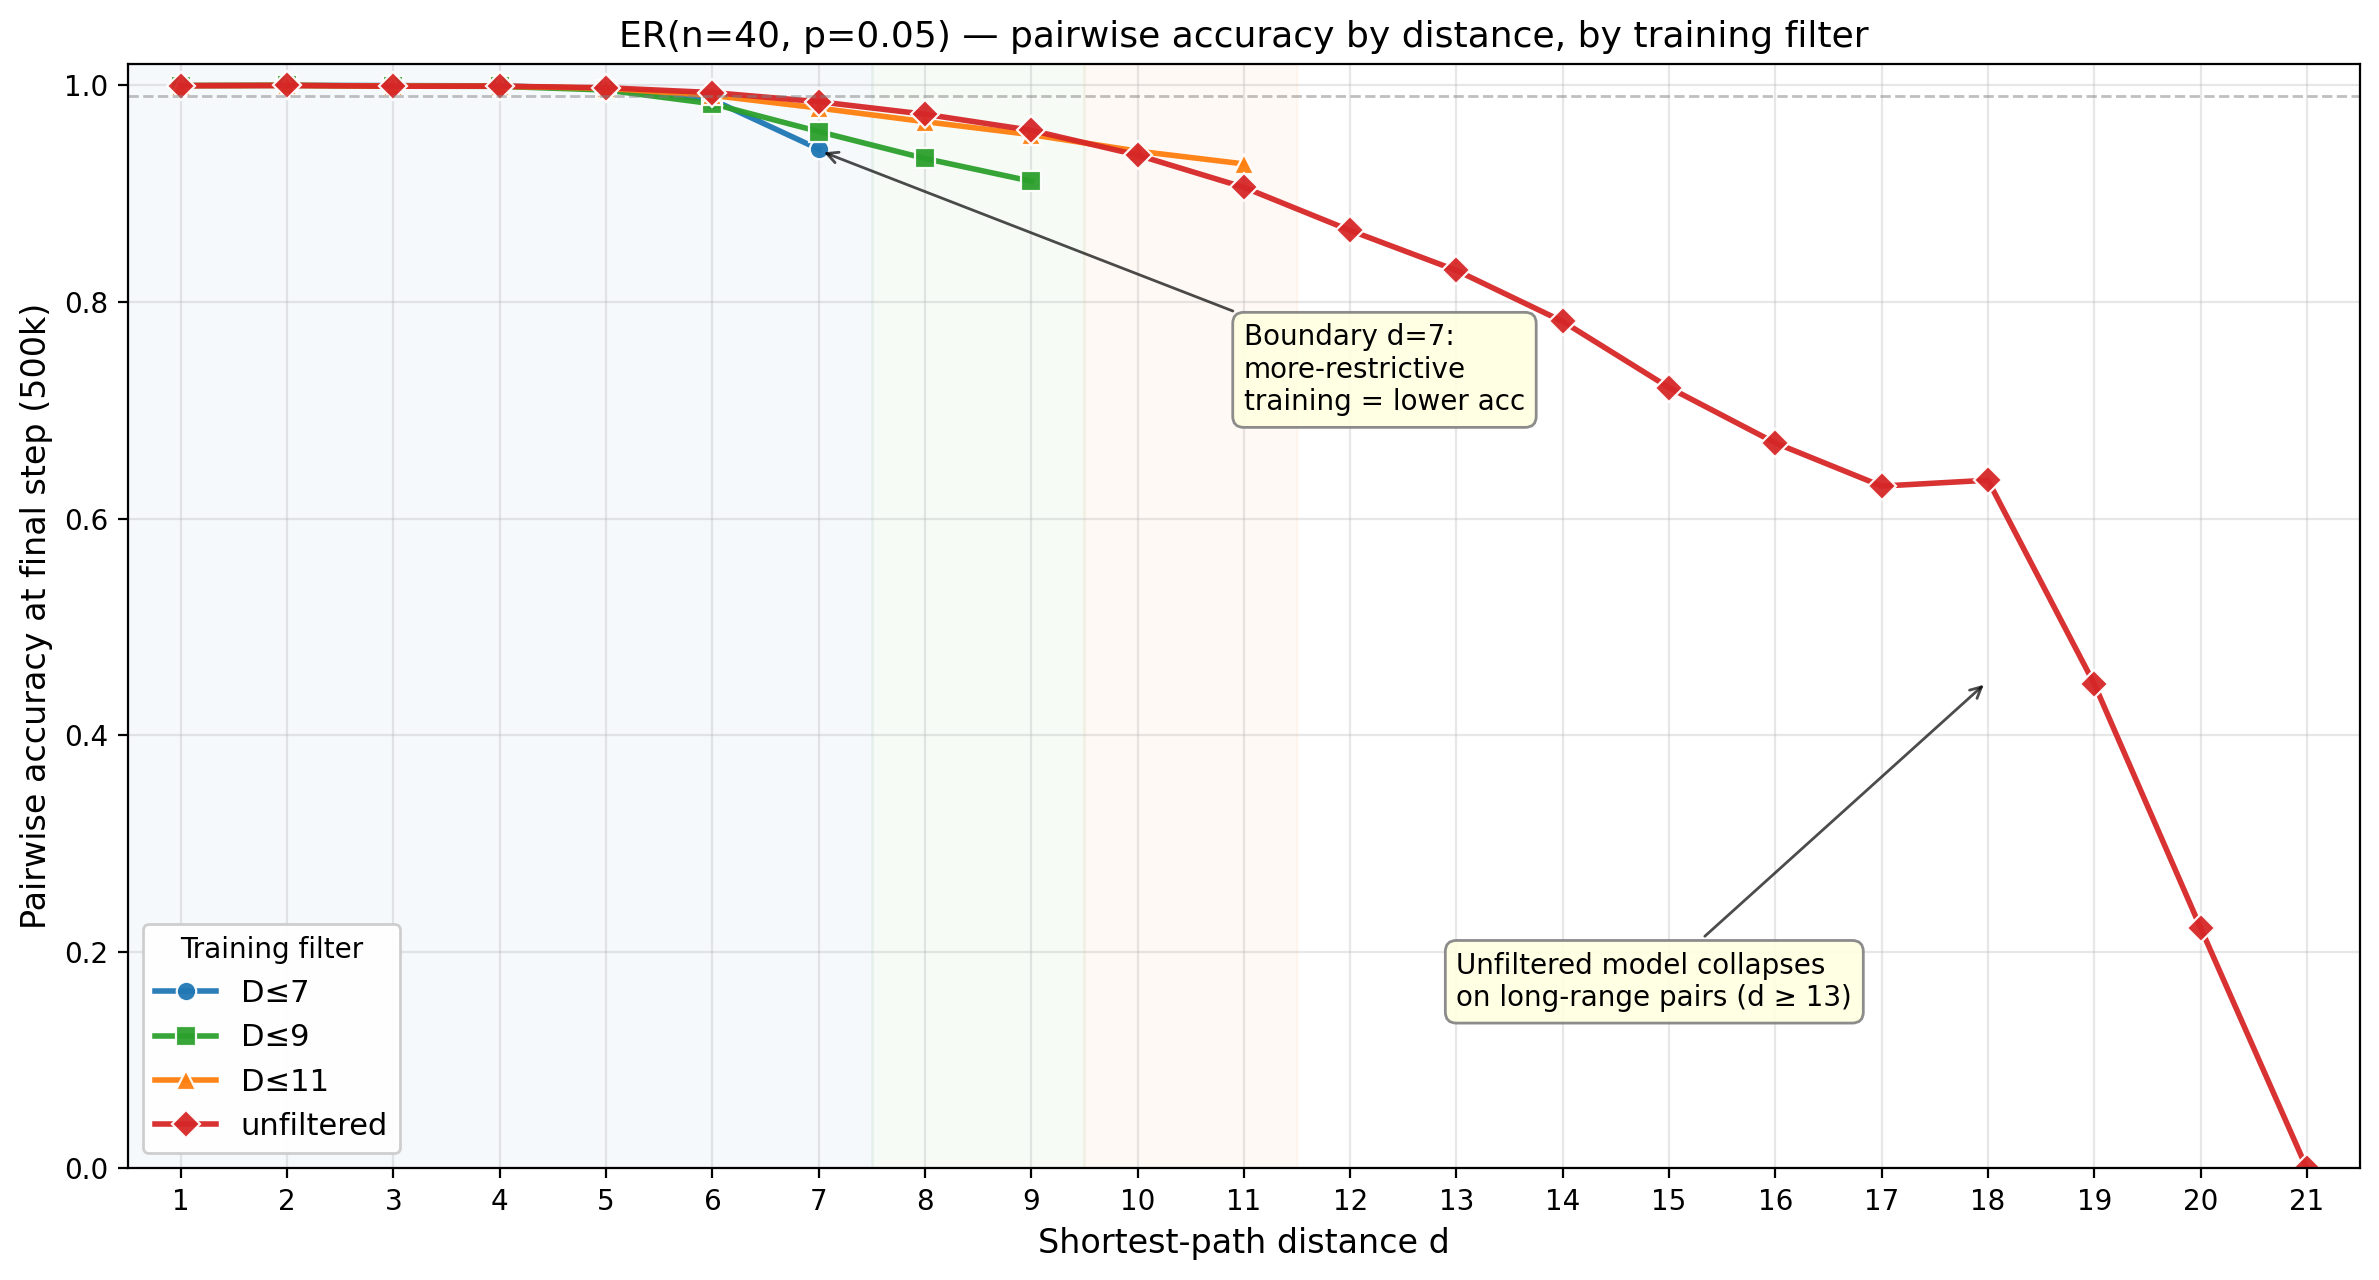
\includegraphics[width=\textwidth]{runs/n40_cross_experiment/02_per_distance.png}
    \caption{Final pairwise accuracy broken down by shortest-path distance
    $d$ for the four diameter-controlled experiments. Background shading
    indicates the support of each filtered training distribution. Each
    curve is truncated at the maximum $d$ present in the corresponding
    test set.}
    \label{fig:n40-perdistance}
\end{figure}

Three observations stand out.

\paragraph{Accuracy is near-perfect at small distances.} For $d \le 5$ all
four models predict pairs correctly with probability greater than
$0.995$ and the four curves are essentially indistinguishable.

\paragraph{Restrictive training is worse at the boundary.} At $d = 7$
the ranking of the four models is the opposite of what one might expect:
unfiltered reaches $0.985$, $D \le 11$ reaches $0.979$, $D \le 9$ reaches
$0.957$, and $D \le 7$ reaches only $0.941$. 

\paragraph{The unfiltered model decays slowly on long-range pairs.} Beyond
$d = 11$, only the unfiltered model has test data on which to be
evaluated; its accuracy drops to $0.83$ at $d = 13$, $0.45$ at $d = 19$
and $0$ at $d = 21$.

\subsection{Cross-experiment view: out-of-distribution}
\label{sec:ch2-cross-ood}

The same four models, evaluated on three OOD test sets ($10{,}000$ graphs
each):
\begin{itemize}
    \item \textbf{2-chains} with $n_{\text{active}} \in \{14, 16, \ldots, 40\}$,
          padded to $40 \times 40$ with isolated nodes;
    \item \textbf{2-cliques} with the same $n_{\text{active}}$ protocol;
    \item \textbf{Unfiltered} ER$(40, 0.05)$ with the per-graph-diameter
          breakdown of exact-match accuracy (for the unfiltered model this
          coincides with the in-distribution evaluation and is reported for
          direct comparison).
\end{itemize}

\subsubsection*{2-chains}

\begin{figure}[H]
    \centering
    
\includegraphics[width=0.9\textwidth]{runs/ood_cross_experiment/ood_cross_chains_per_distance.png}
    \caption{2-chains OOD: pairwise accuracy as a function of the
    chain-internal distance $d$, compared across the four diameter-controlled
    small-model runs. Each curve is averaged over all $n_{\text{active}}$
    values.}
    \label{fig:ood-chains-perdist-small}
\end{figure}

Exact match is $0$ for all four models. Average pairwise accuracy on the
$\sim 3.7$M chain-internal reachable pairs is:
\begin{itemize}
    \item Unfiltered: $0.636$
    \item $D \le 9$: $0.597$
    \item $D \le 7$: $0.577$
    \item $D \le 11$: $0.526$
\end{itemize}
The unfiltered model is the most robust on chain transfer despite never
having been trained on a chain. The diameter-restricted models drop to
zero accuracy at, or even before, their respective training cut-offs.

\subsubsection*{2-cliques}

Three of the four models reach exact match $0$. The only exception is the
$D \le 7$ model, which scores $0.068$ overall: this signal comes entirely
from the $n_{\text{active}} = 14$ subset (two $7$-cliques padded with $26$
isolated nodes) where the model achieves $100\%$ exact match, and is $0$
for every other $n_{\text{active}}$. Per-distance accuracy across all four
models is essentially the same as in the small-scale 2-cliques OOD test
(Chapter~\ref{sec:ch1}): $d = 1$ accuracy is very low ($\le 0.08$) and the
``disconnected'' bin dominates the pairwise number.

\subsubsection*{Unfiltered ER, by graph diameter}

\begin{figure}[H]
    \centering
    
\includegraphics[width=\textwidth]{runs/ood_cross_experiment/ood_cross_per_diam_bucket.png}
    \caption{OOD evaluation on unfiltered ER$(40, 0.05)$: exact-match
    accuracy broken down by the diameter of the test graph, compared
    across the four diameter-controlled small-model runs.}
    \label{fig:ood-cross-perdiam-small}
\end{figure}

\begin{table}[H]
\centering
\begin{tabular}{lccccc}
\toprule
Model       & $D \le 7$ & $D \le 9$ & $D \le 11$ & $D > 11$ & overall \\
\midrule
Unfiltered  & 0.734 & 0.820 & 0.826 & \textbf{0.687} & 0.806 \\
$D \le 11$  & 0.765 & 0.828 & 0.800 & 0.329 & 0.732 \\
$D \le 9$   & 0.758 & 0.792 & 0.697 & 0.107 & 0.612 \\
$D \le 7$   & \textbf{0.803} & 0.580 & 0.405 & 0.003 & 0.347 \\
\bottomrule
\end{tabular}
\caption{Exact-match accuracy on a fixed test set of $10{,}000$
unfiltered ER$(40, 0.05)$ graphs, broken down by the test-graph diameter
(number of graphs per bucket: $1{,}329$, $5{,}574$, $8{,}548$, $1{,}452$).
Bold entries mark the best model in each column.}
\label{tab:ood-er-buckets-small}
\end{table}

Three patterns:
\begin{itemize}
    \item Each diameter-restricted model wins on the bucket that matches its
          training distribution and the unfiltered model wins on the
          tail bucket $D > 11$.
    \item The tighter the filter, the more catastrophic the failure on the
          excluded bucket: $0.329$ for $D \le 11$, $0.107$ for $D \le 9$,
          $0.003$ for $D \le 7$.
    \item Even on buckets nominally inside every model's training
          distribution (e.g.\ $D \le 7$, $D \le 9$), the unfiltered model
          is competitive with or better than the corresponding specialist.
\end{itemize}

\subsection{Per-experiment figures (small model)}

The following four subsections collect, for each filter, the in-distribution
training curves and the per-experiment OOD plots that were aggregated in
the cross-experiment view above. The text is intentionally short.

\subsubsection{Unfiltered}

\begin{figure}[H]
    \centering
    \begin{subfigure}[t]{0.32\textwidth}
        \centering
        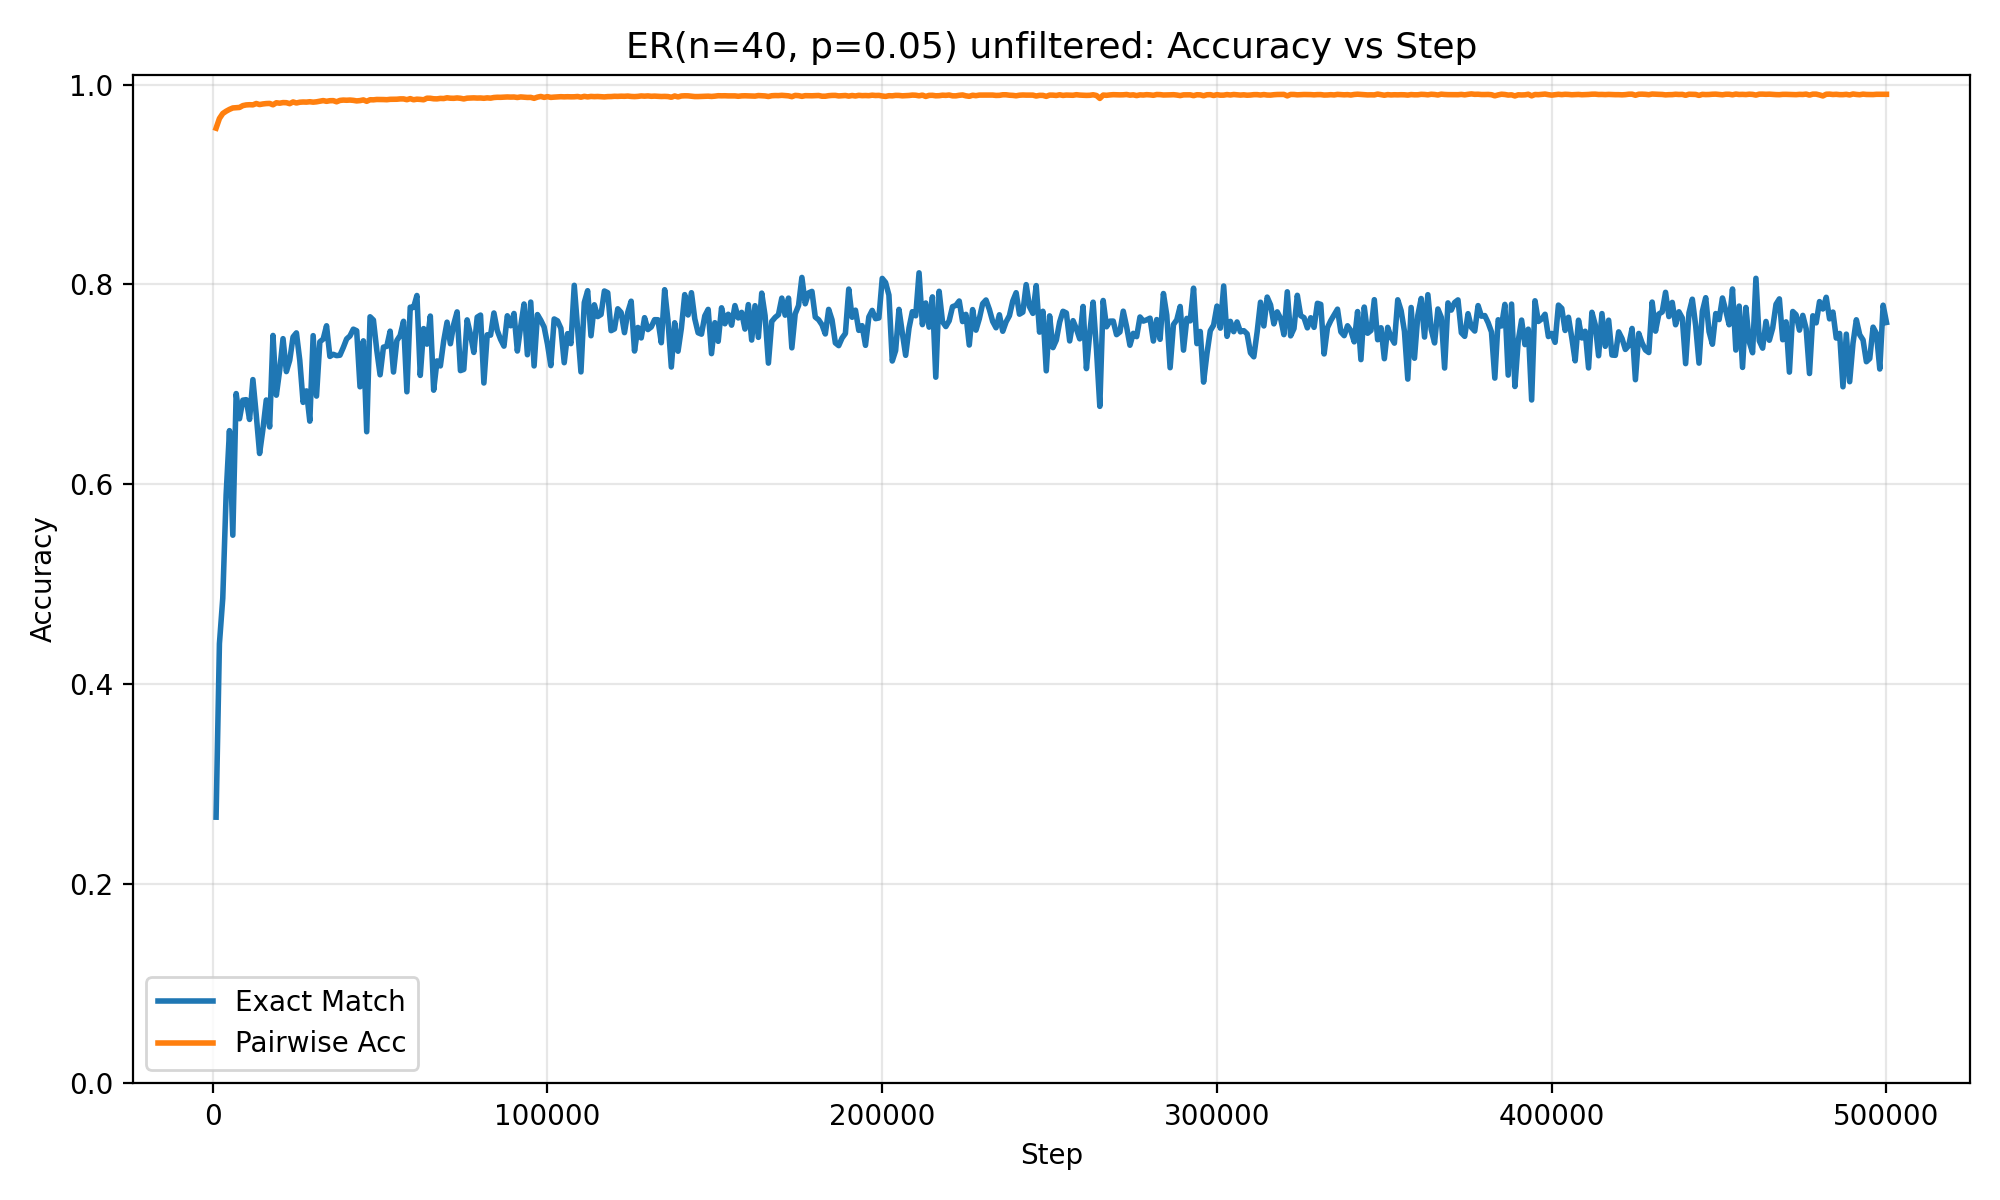
\includegraphics[width=\textwidth]{runs/retrain_er_n40_485350/n40_p005_unfiltered/er_n40_unfiltered_accuracy.png}
        \caption{Exact match and pairwise accuracy.}
    \end{subfigure}
    \hfill
    \begin{subfigure}[t]{0.32\textwidth}
        \centering
        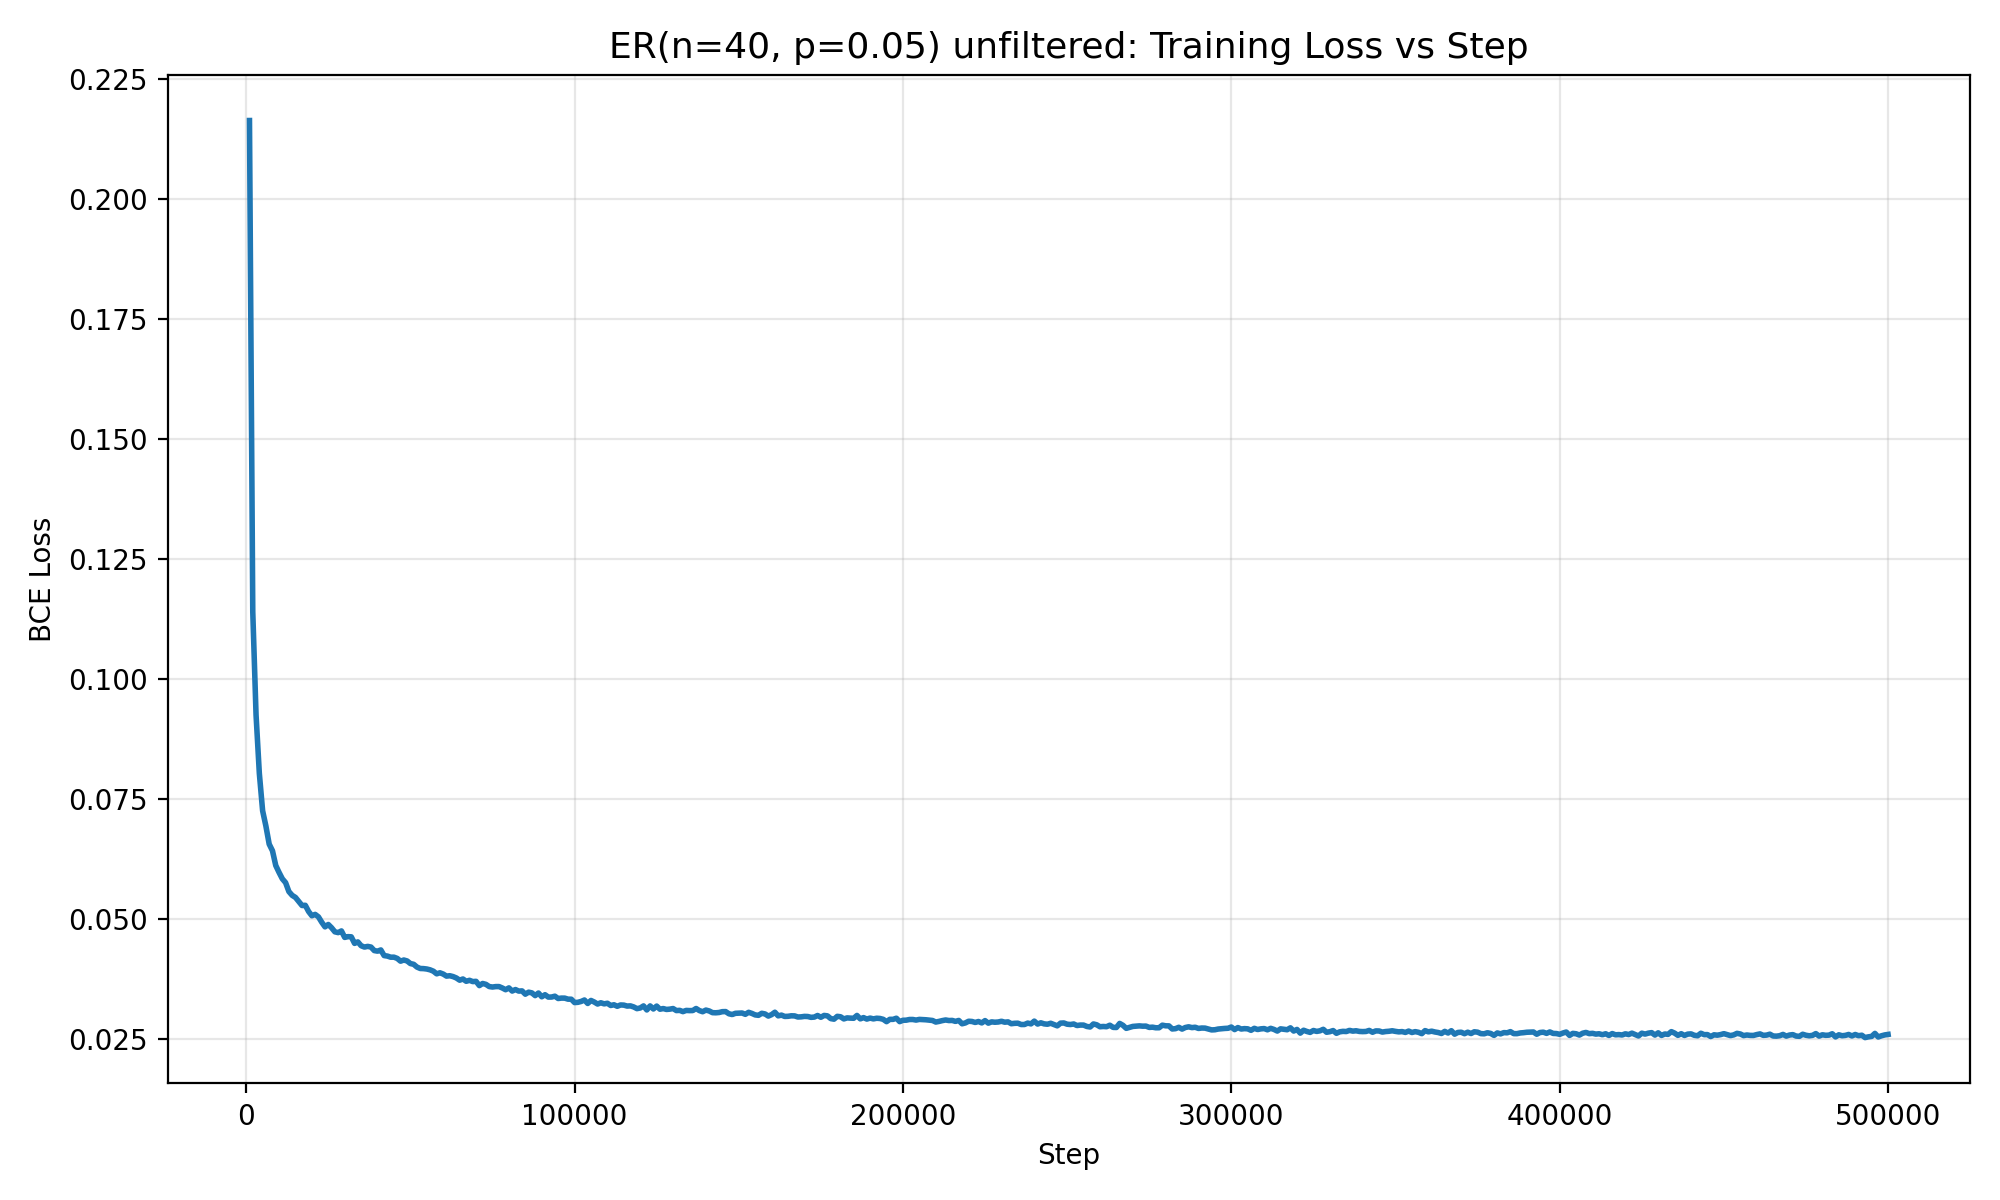
\includegraphics[width=\textwidth]{runs/retrain_er_n40_485350/n40_p005_unfiltered/er_n40_unfiltered_loss.png}
        \caption{Training loss.}
    \end{subfigure}
    \hfill
    \begin{subfigure}[t]{0.32\textwidth}
        \centering
        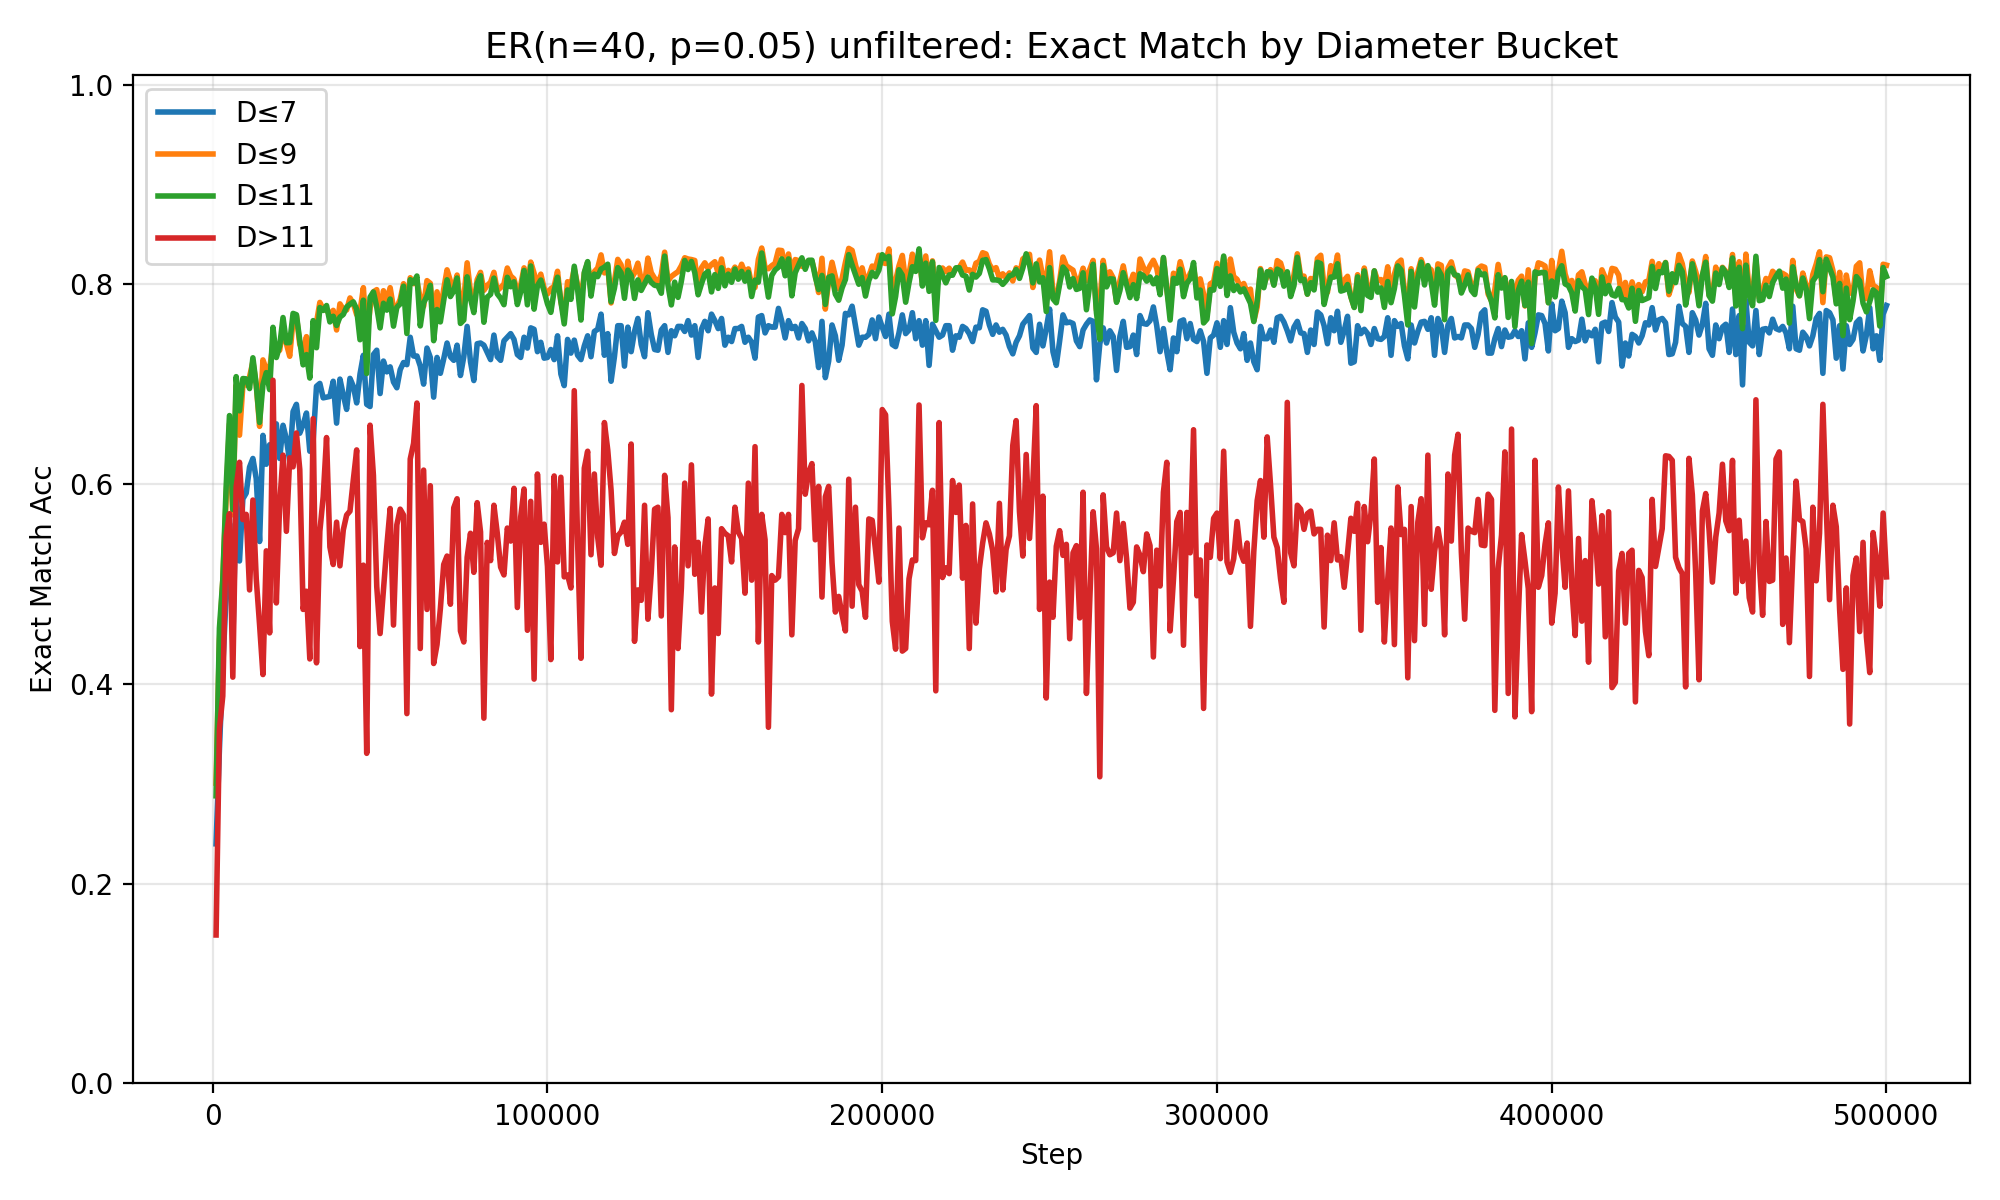
\includegraphics[width=\textwidth]{runs/retrain_er_n40_485350/n40_p005_unfiltered/er_n40_unfiltered_per_diam_bucket.png}
        \caption{Exact match per test-graph diameter bucket.}
    \end{subfigure}

    \vspace{1em}

    \begin{subfigure}[t]{0.6\textwidth}
        \centering
        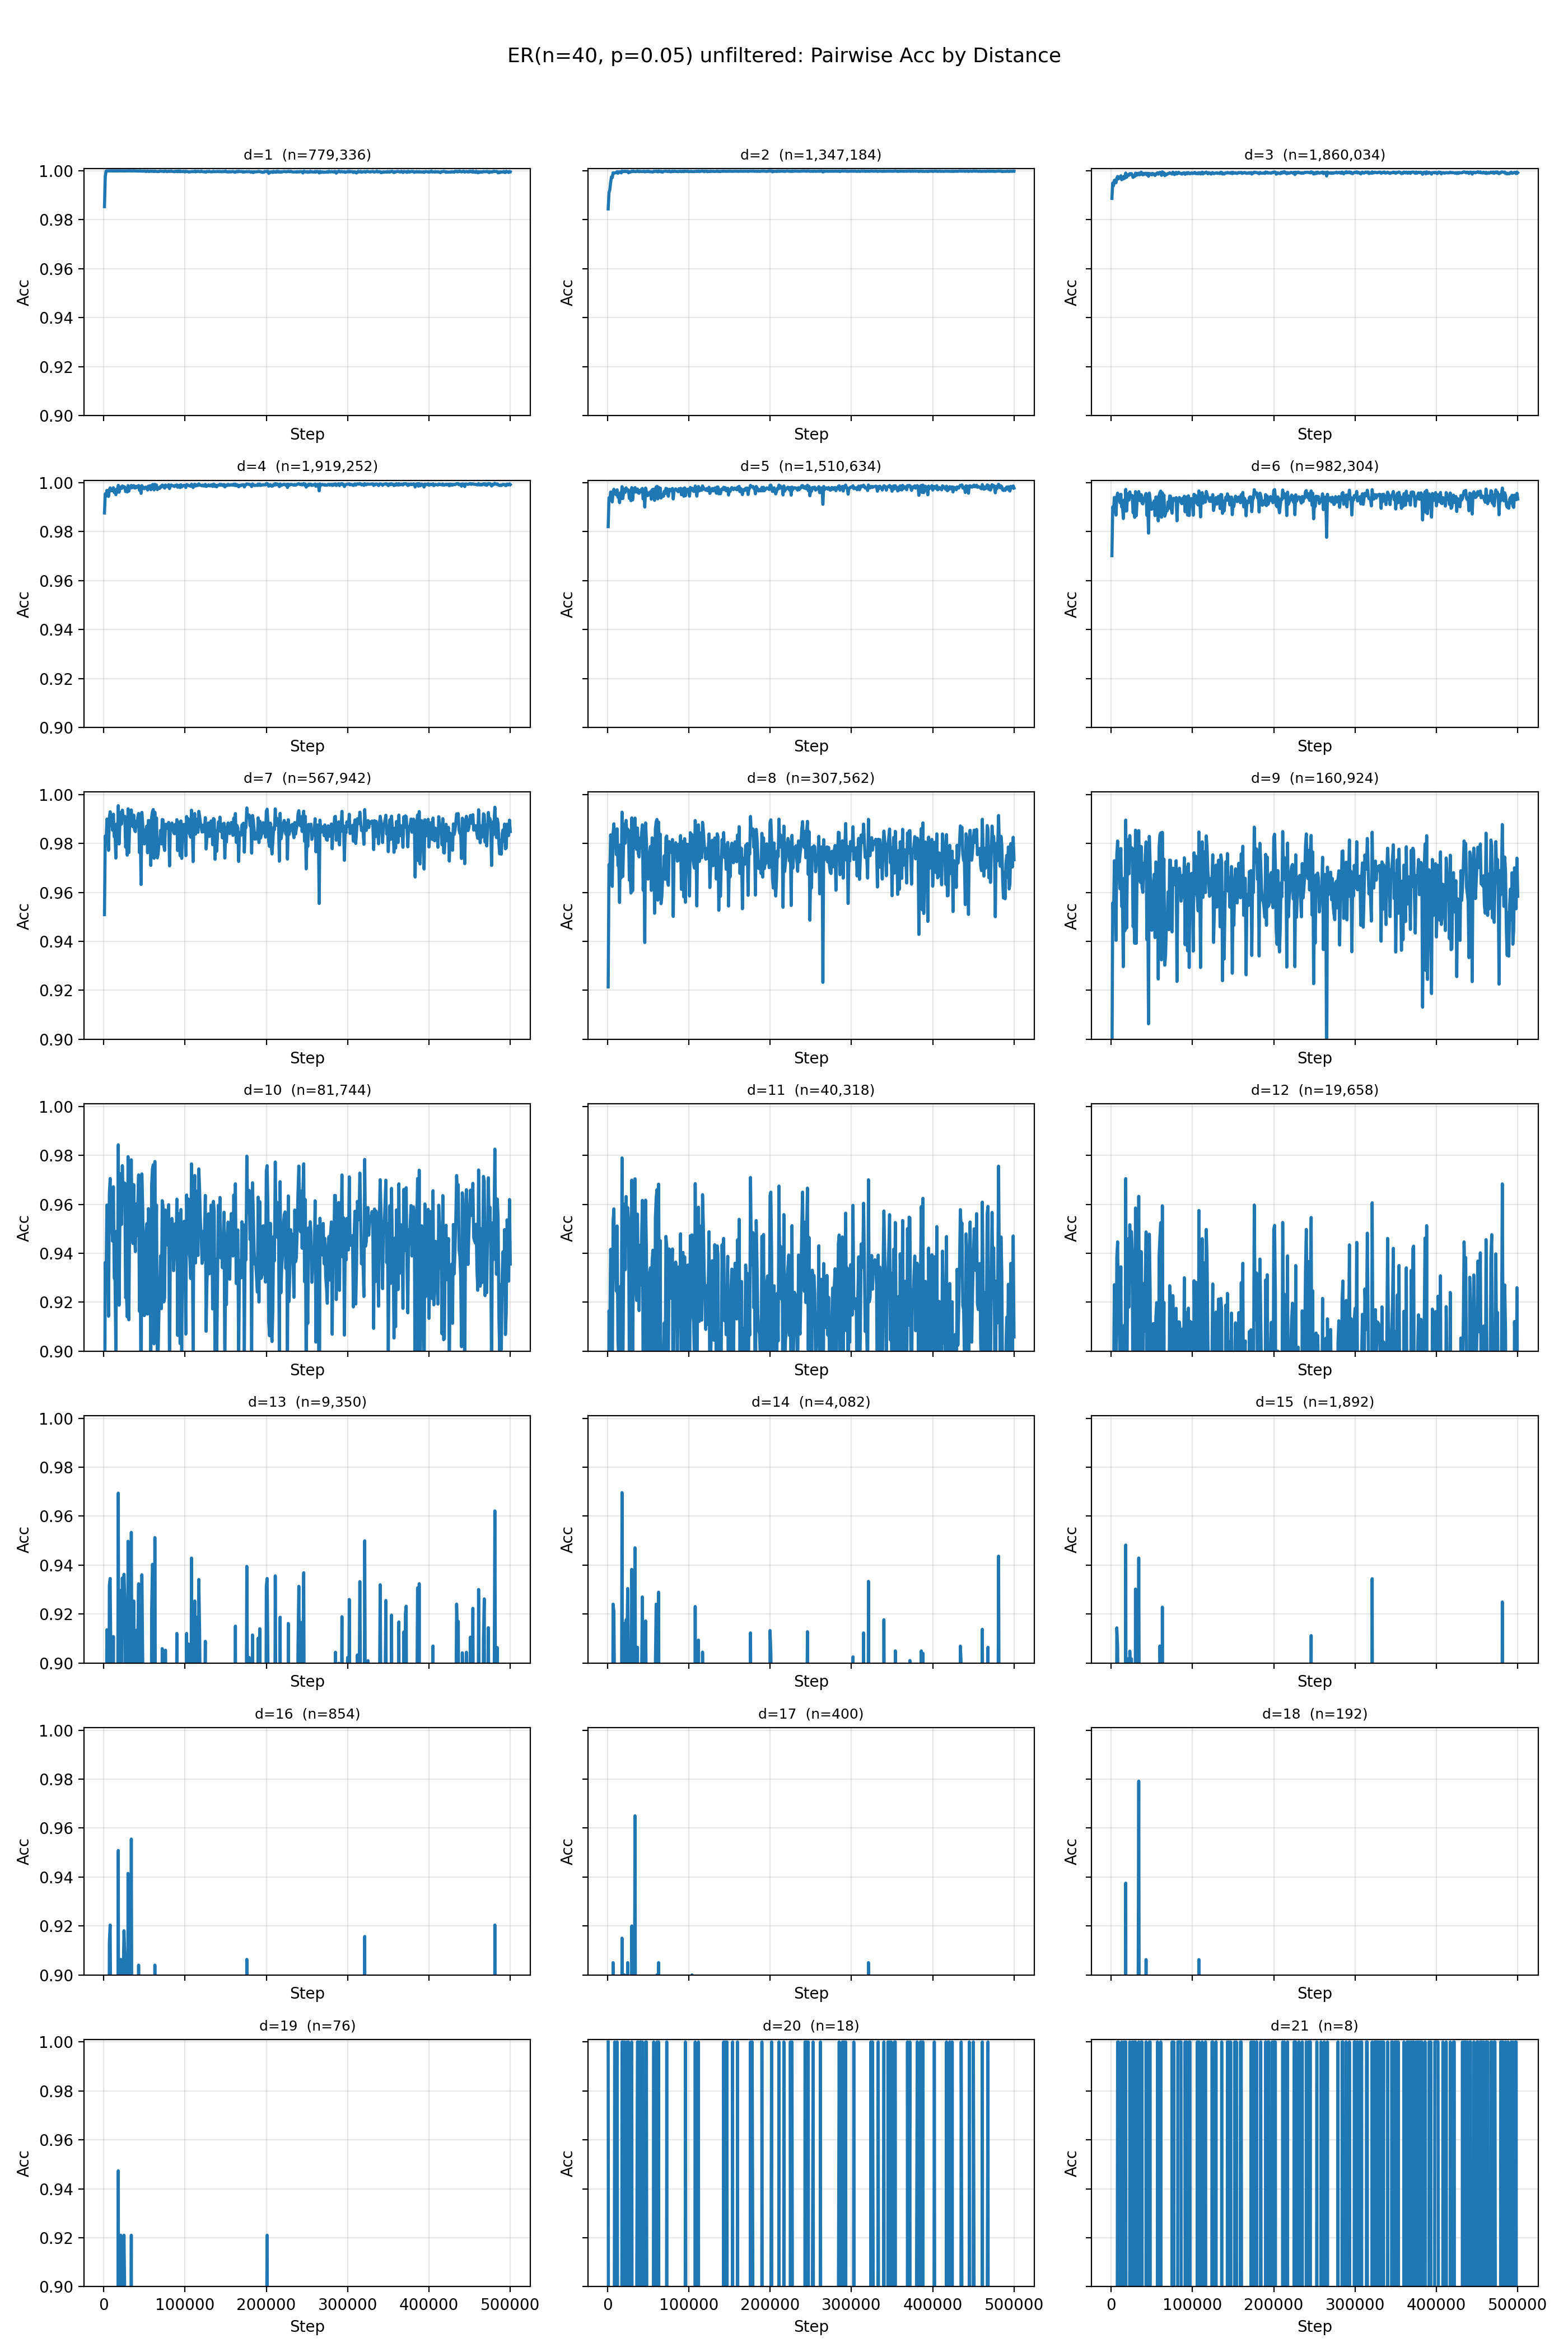
\includegraphics[width=\textwidth]{runs/retrain_er_n40_485350/n40_p005_unfiltered/er_n40_unfiltered_per_dist_sm.png}
        \caption{Pairwise accuracy by shortest-path distance. The number above each panel is the count of test pairs at that distance.}
    \end{subfigure}

    \caption{Unfiltered, in distribution.}
\end{figure}

\begin{figure}[H]
    \centering
    \begin{subfigure}[t]{0.66\textwidth}
        \centering
        
\includegraphics[width=\textwidth]{runs/ood_cross_experiment/ood_n40_unfiltered_per_distance_bars.png}
        \caption{Per-distance pairwise accuracy on the three OOD sets.}
    \end{subfigure}
    \hfill
    \begin{subfigure}[t]{0.32\textwidth}
        \centering
        
\includegraphics[width=\textwidth]{runs/ood_cross_experiment/ood_n40_unfiltered_per_diam_bucket.png}
        \caption{Exact match on unfiltered ER by diameter bucket.}
    \end{subfigure}
    \caption{Unfiltered, OOD.}
\end{figure}

\subsubsection{$D \le 11$}

\begin{figure}[H]
    \centering
    \begin{subfigure}[t]{0.32\textwidth}
        \centering
        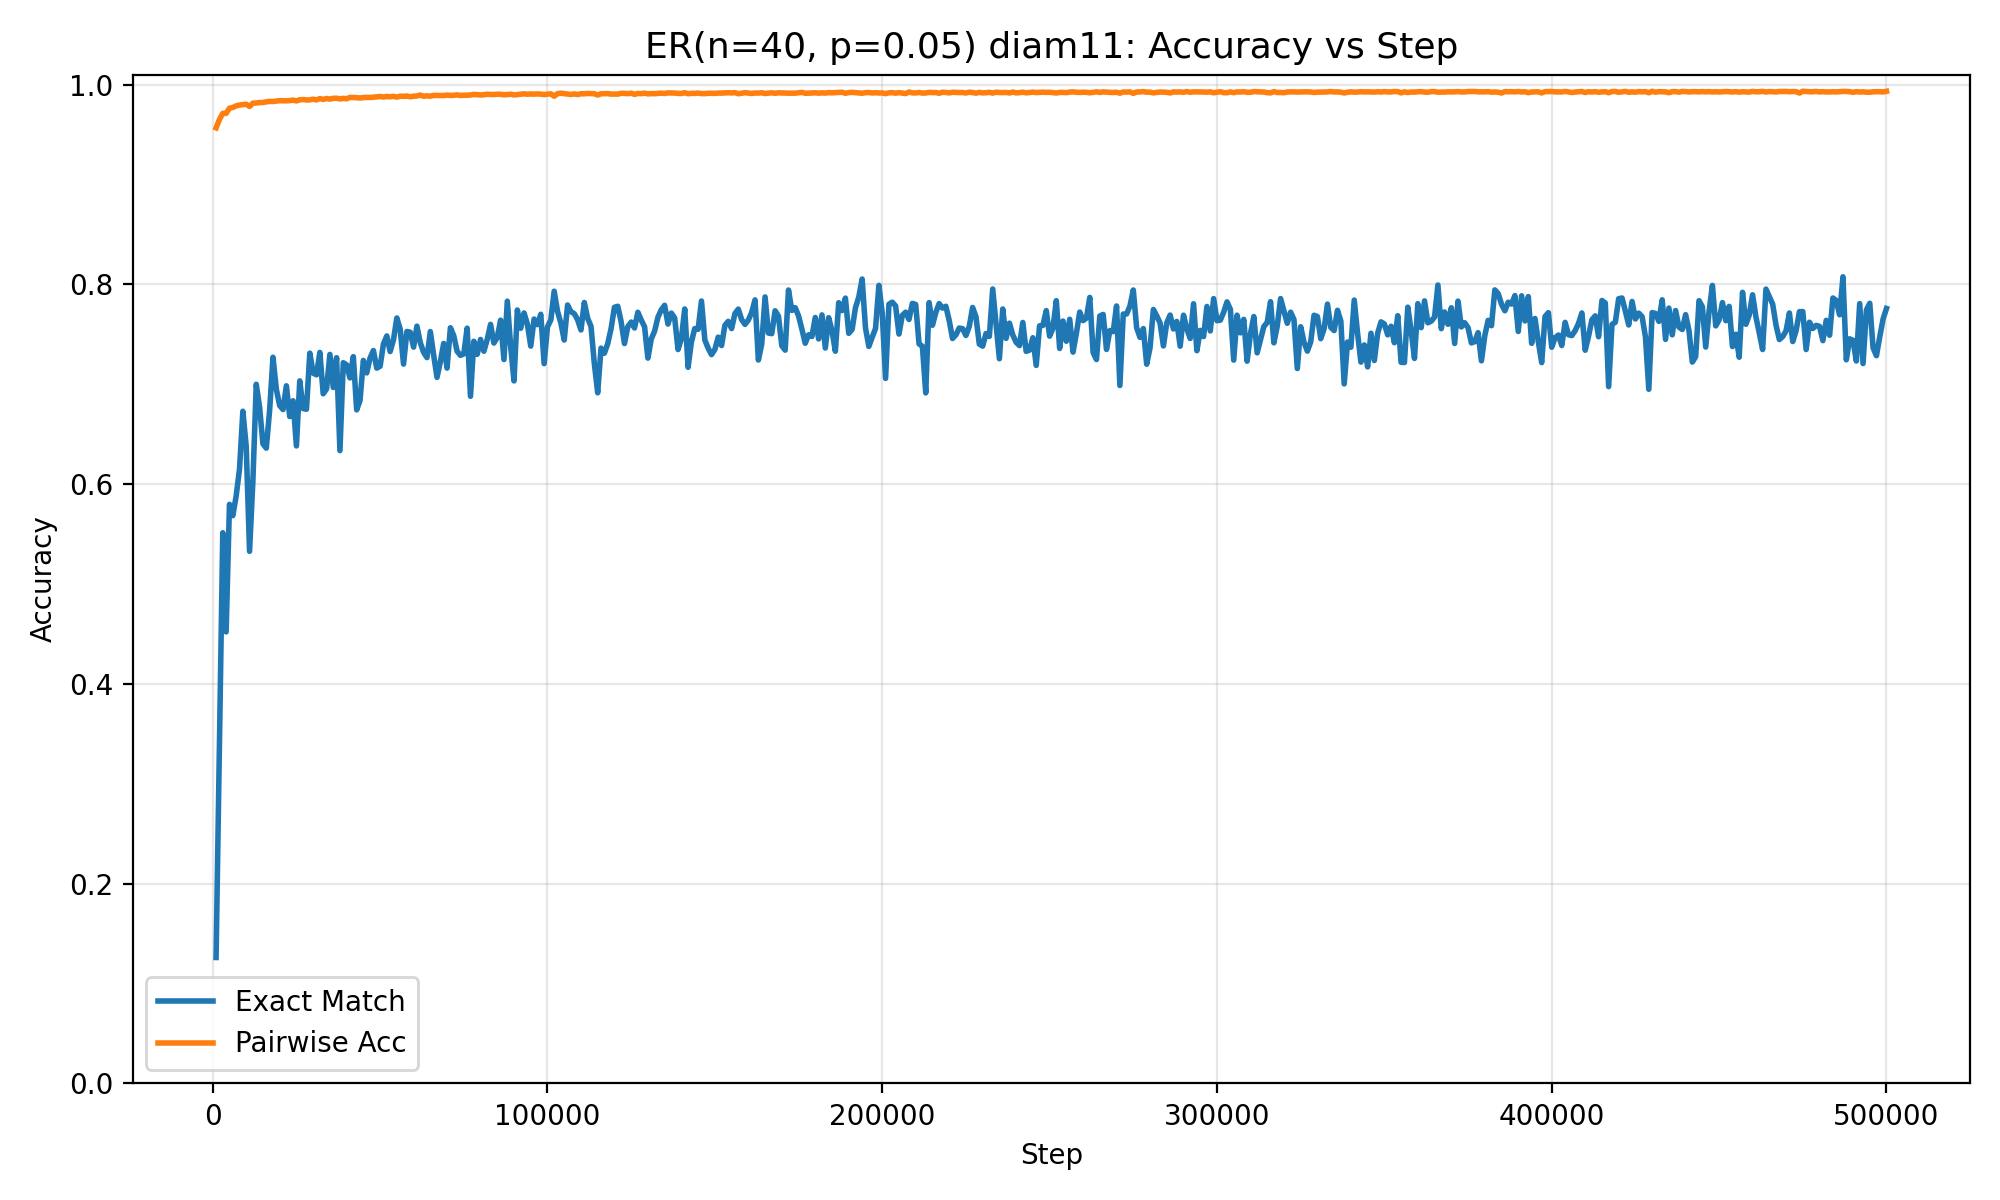
\includegraphics[width=\textwidth]{runs/retrain_er_n40_485352/n40_p005_diam11/er_n40_diam11_accuracy.png}
        \caption{Exact match and pairwise accuracy.}
    \end{subfigure}
    \hfill
    \begin{subfigure}[t]{0.32\textwidth}
        \centering
        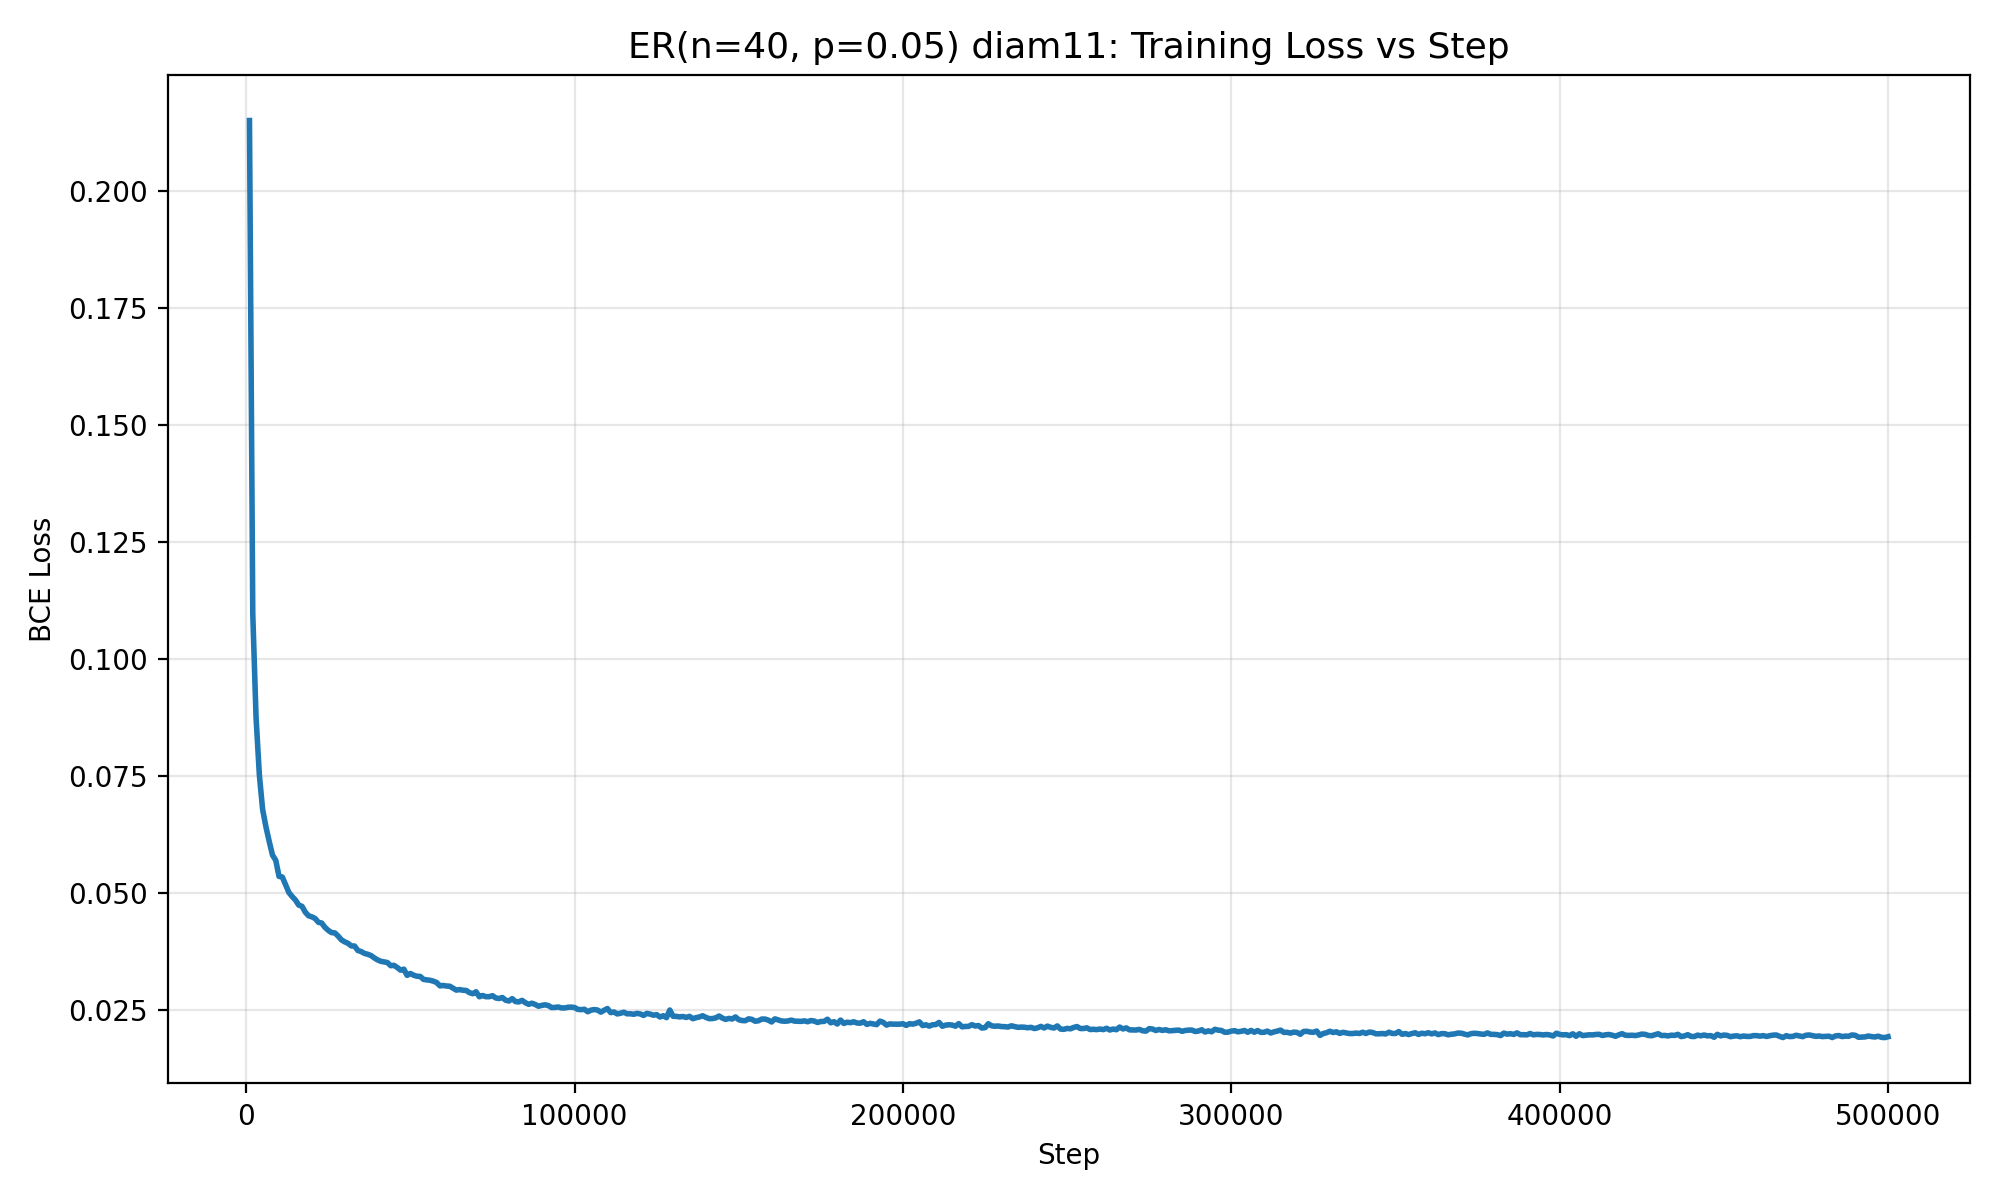
\includegraphics[width=\textwidth]{runs/retrain_er_n40_485352/n40_p005_diam11/er_n40_diam11_loss.png}
        \caption{Training loss.}
    \end{subfigure}
    \hfill
    \begin{subfigure}[t]{0.32\textwidth}
        \centering
        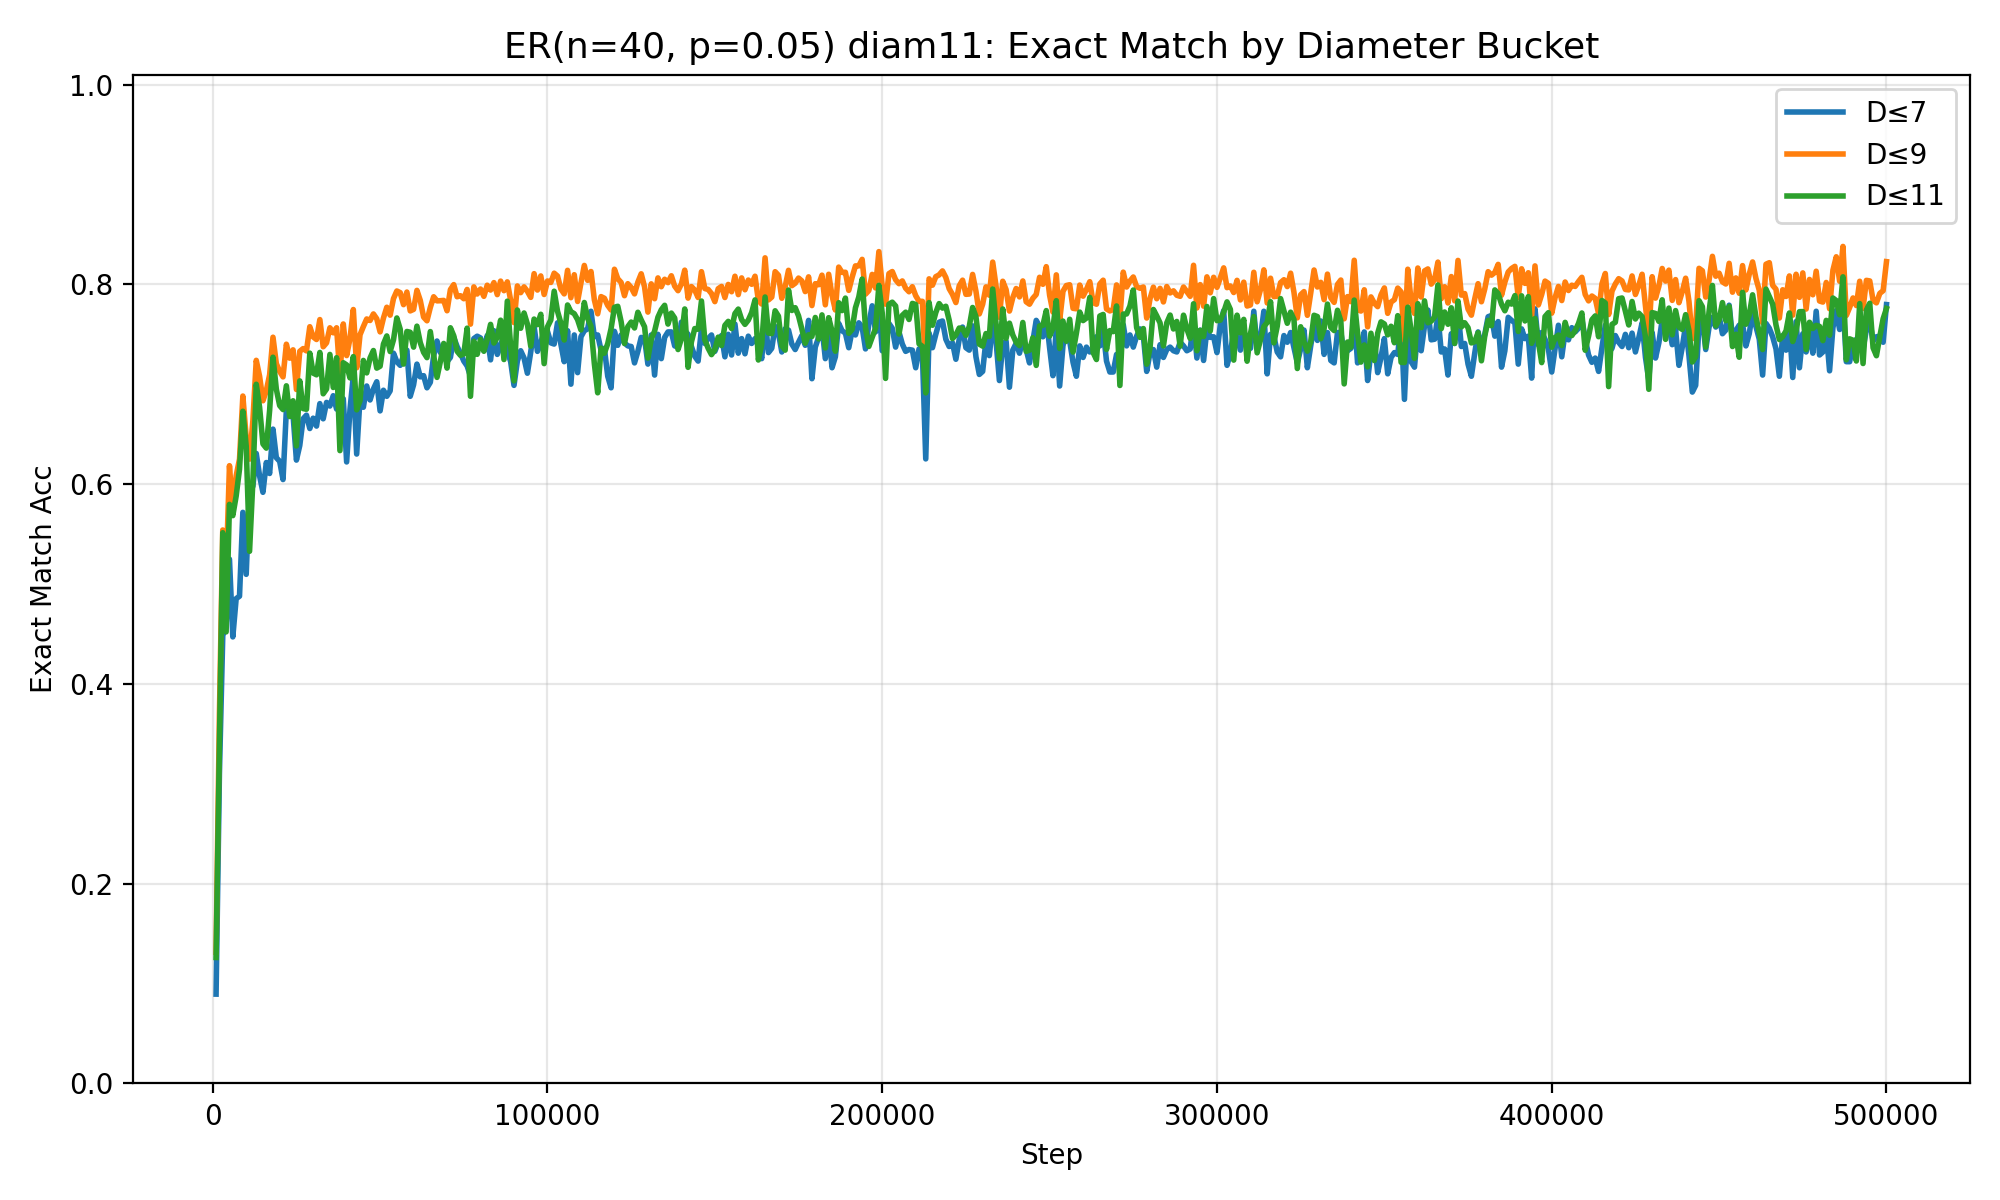
\includegraphics[width=\textwidth]{runs/retrain_er_n40_485352/n40_p005_diam11/er_n40_diam11_per_diam_bucket.png}
        \caption{Exact match per test-graph diameter bucket.}
    \end{subfigure}

    \vspace{1em}

    \begin{subfigure}[t]{0.6\textwidth}
        \centering
        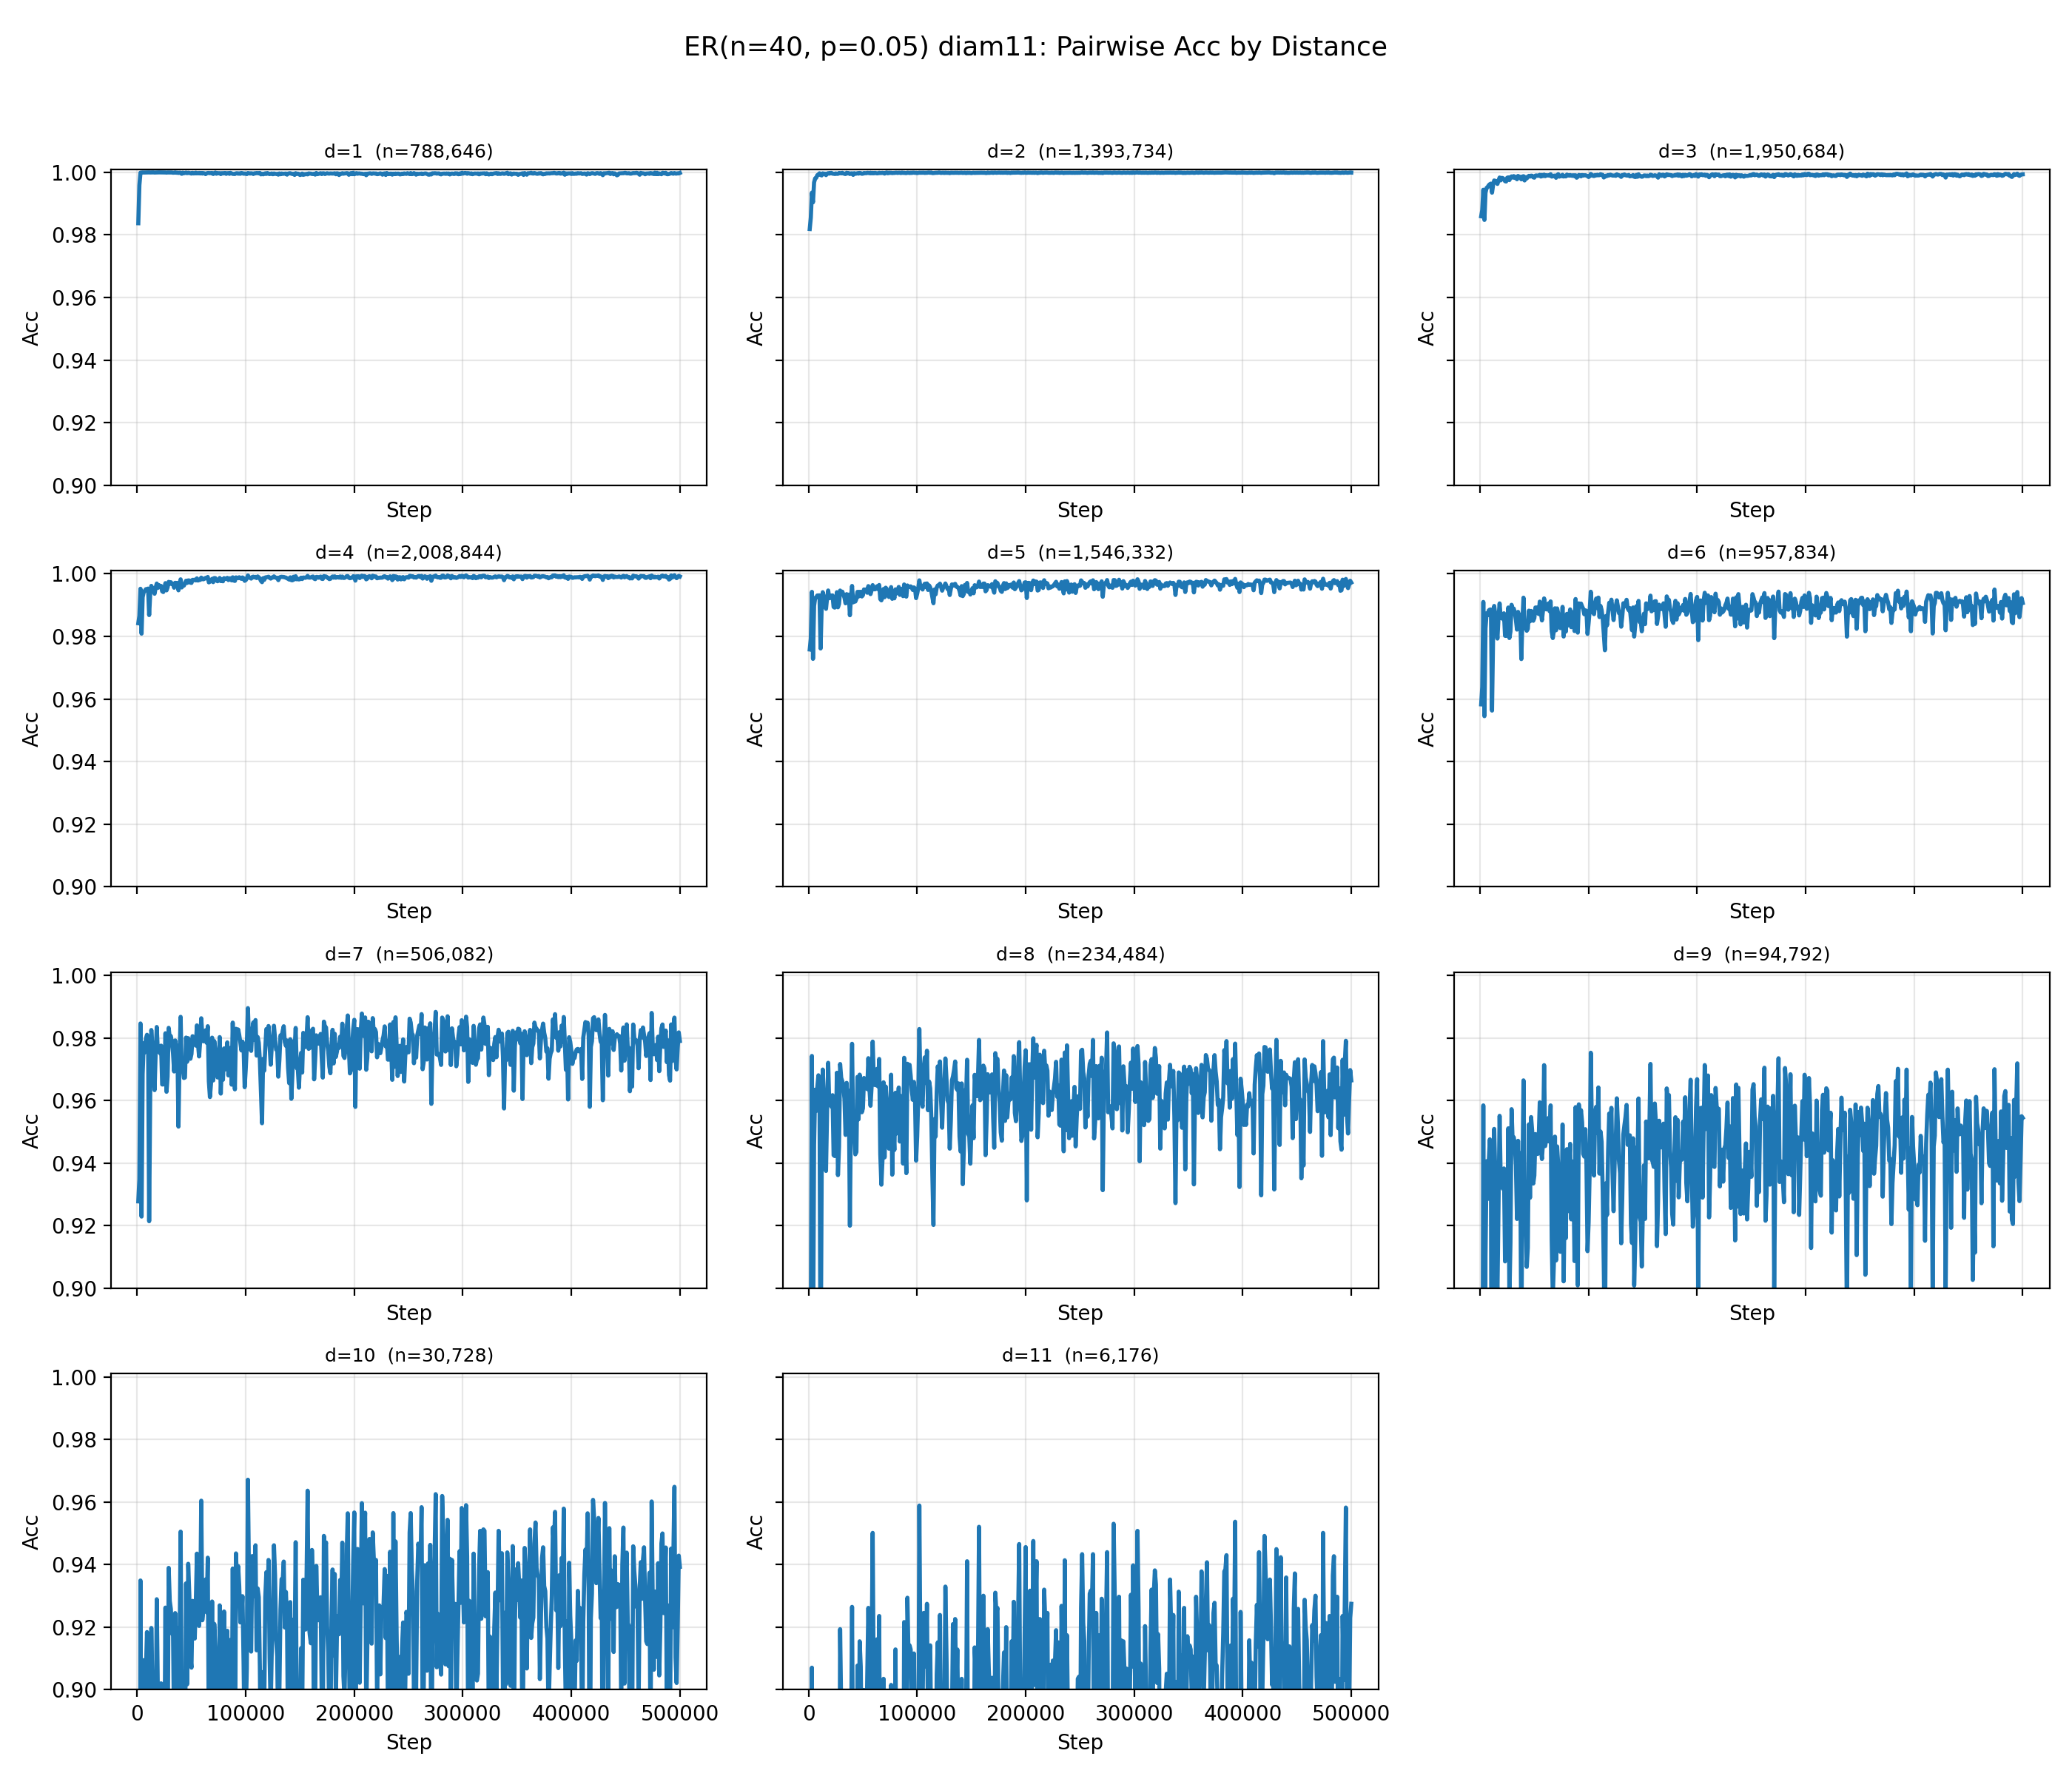
\includegraphics[width=\textwidth]{runs/retrain_er_n40_485352/n40_p005_diam11/er_n40_diam11_per_dist_sm.png}
        \caption{Pairwise accuracy by shortest-path distance. The number above each panel is the count of test pairs at that distance.}
    \end{subfigure}

    \caption{$D \le 11$, in distribution.}
\end{figure}

\begin{figure}[H]
    \centering
    \begin{subfigure}[t]{0.66\textwidth}
        \centering
        
\includegraphics[width=\textwidth]{runs/ood_cross_experiment/ood_n40_diam11_per_distance_bars.png}
        \caption{Per-distance pairwise accuracy on the three OOD sets.}
    \end{subfigure}
    \hfill
    \begin{subfigure}[t]{0.32\textwidth}
        \centering
        
\includegraphics[width=\textwidth]{runs/ood_cross_experiment/ood_n40_diam11_per_diam_bucket.png}
        \caption{Exact match on unfiltered ER by diameter bucket.}
    \end{subfigure}
    \caption{$D \le 11$, OOD.}
\end{figure}

\subsubsection{$D \le 9$}

\begin{figure}[H]
    \centering
    \begin{subfigure}[t]{0.32\textwidth}
        \centering
        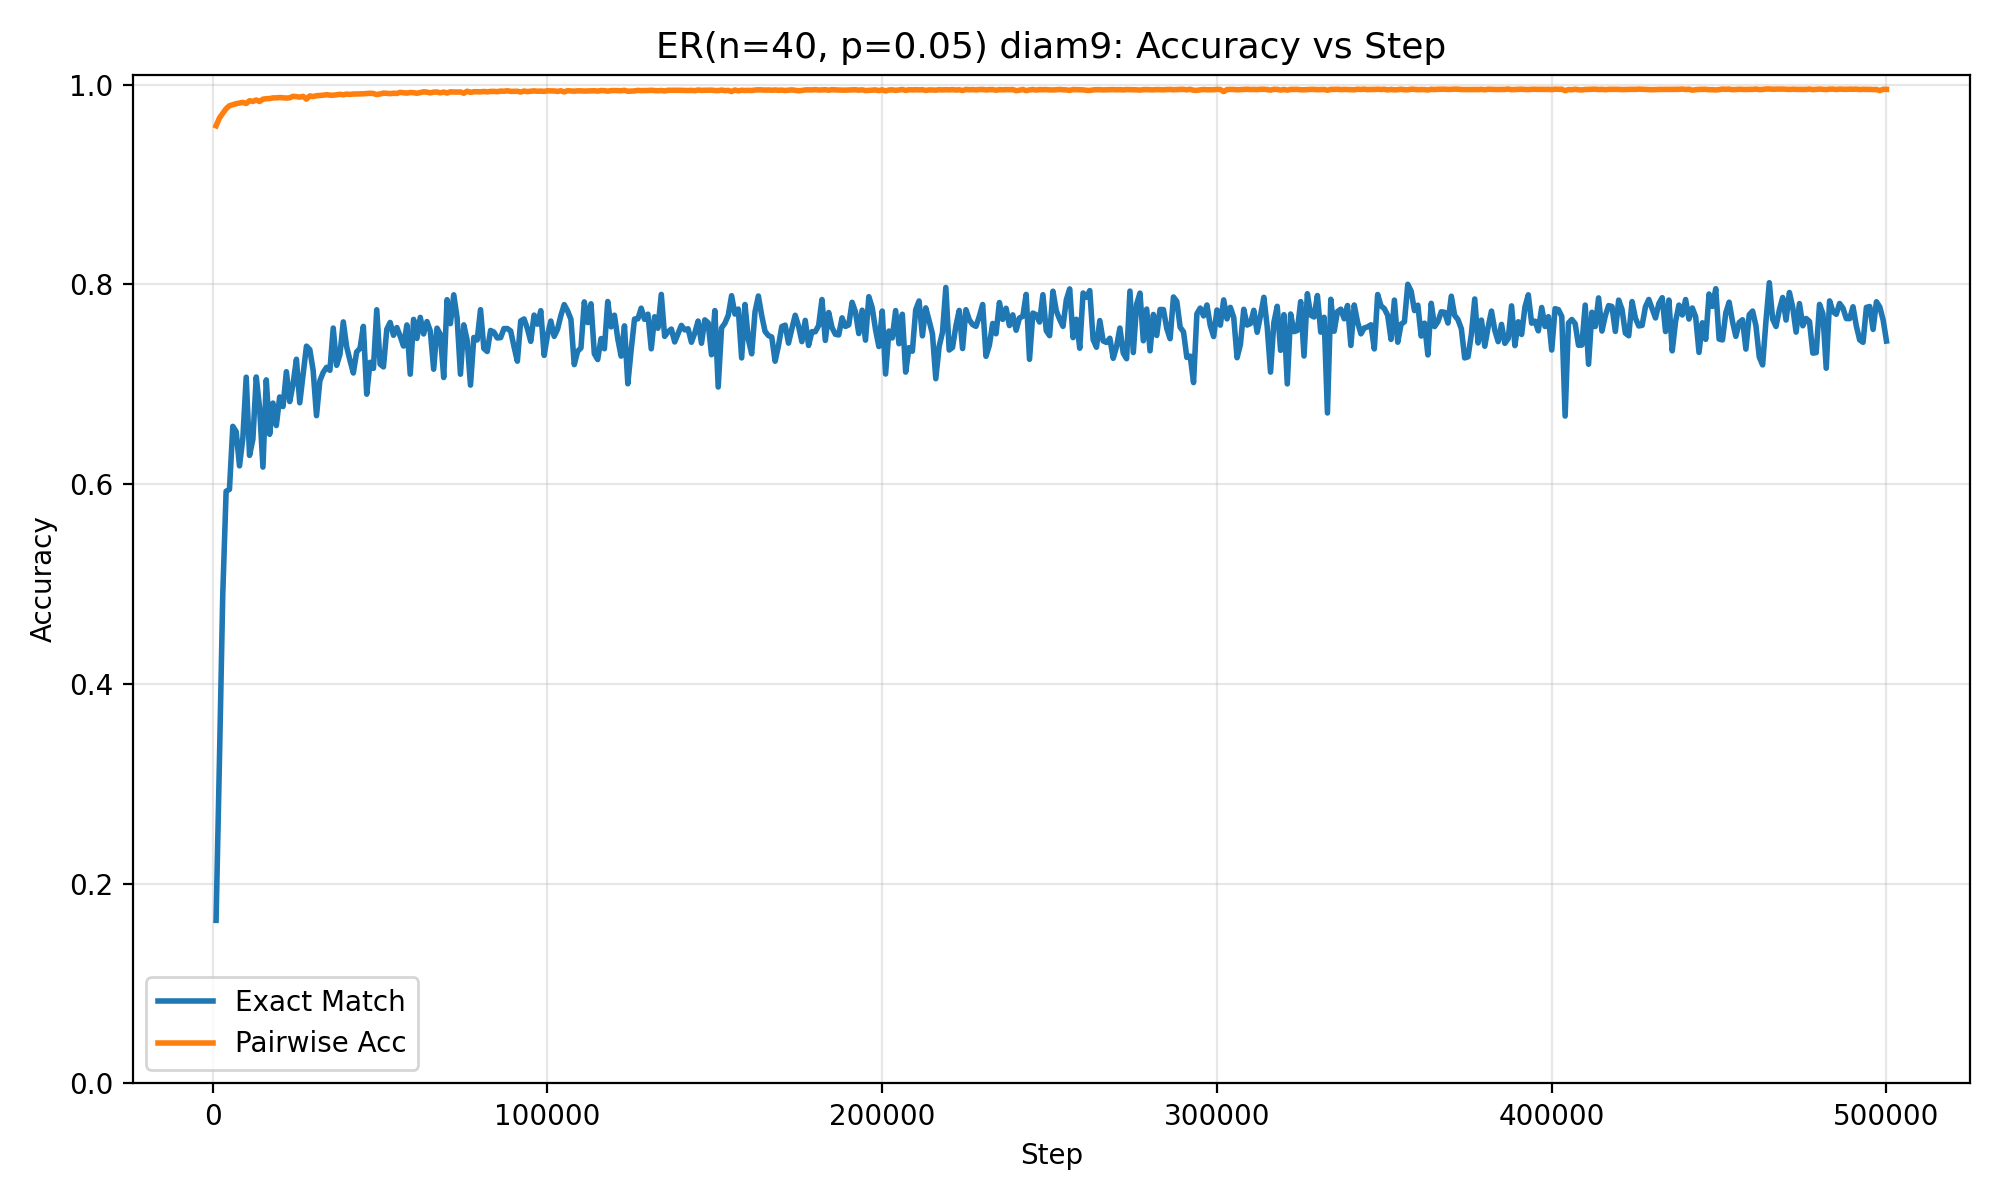
\includegraphics[width=\textwidth]{runs/retrain_er_n40_485351/n40_p005_diam9/er_n40_diam9_accuracy.png}
        \caption{Exact match and pairwise accuracy.}
    \end{subfigure}
    \hfill
    \begin{subfigure}[t]{0.32\textwidth}
        \centering
        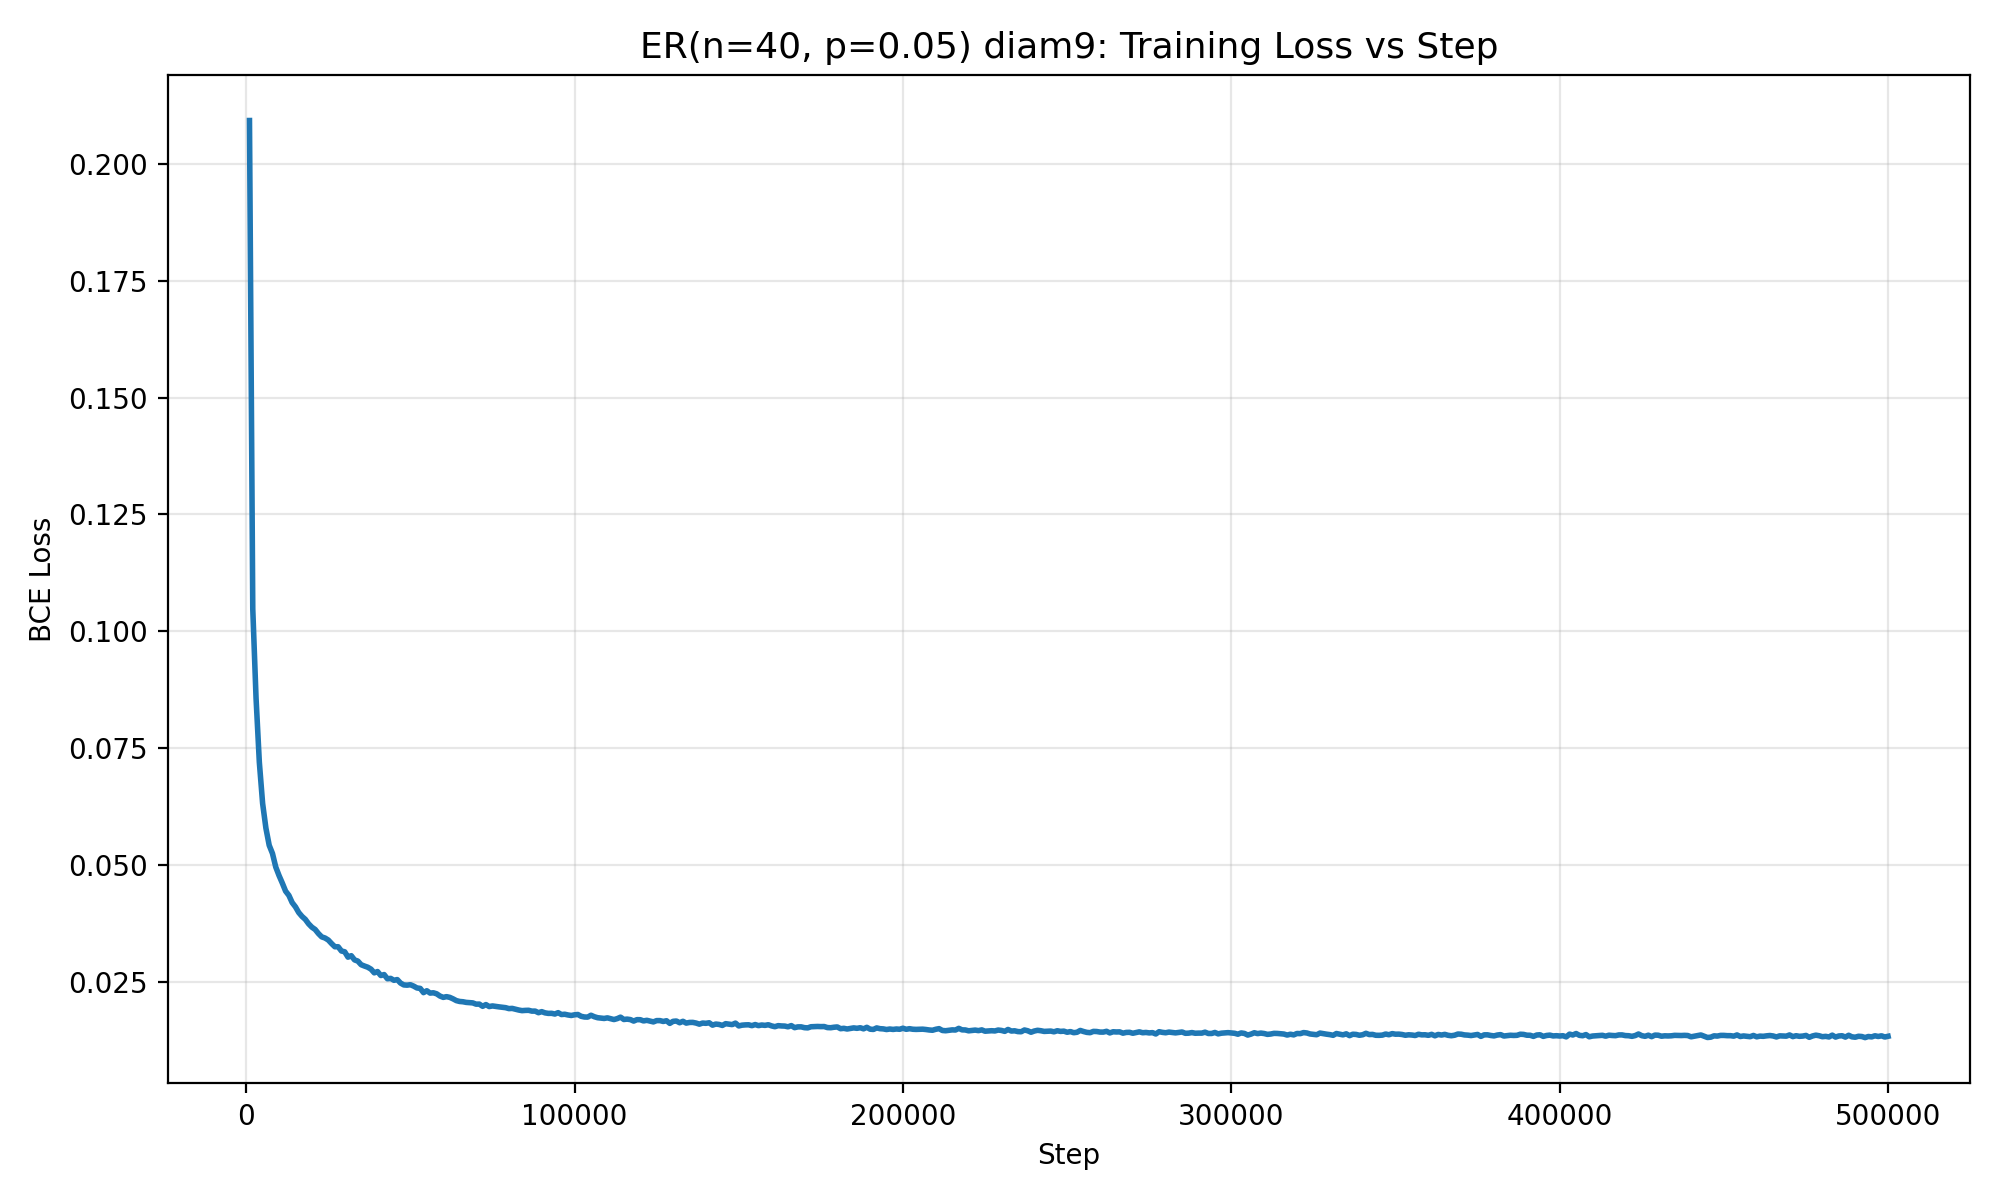
\includegraphics[width=\textwidth]{runs/retrain_er_n40_485351/n40_p005_diam9/er_n40_diam9_loss.png}
        \caption{Training loss.}
    \end{subfigure}
    \hfill
    \begin{subfigure}[t]{0.32\textwidth}
        \centering
        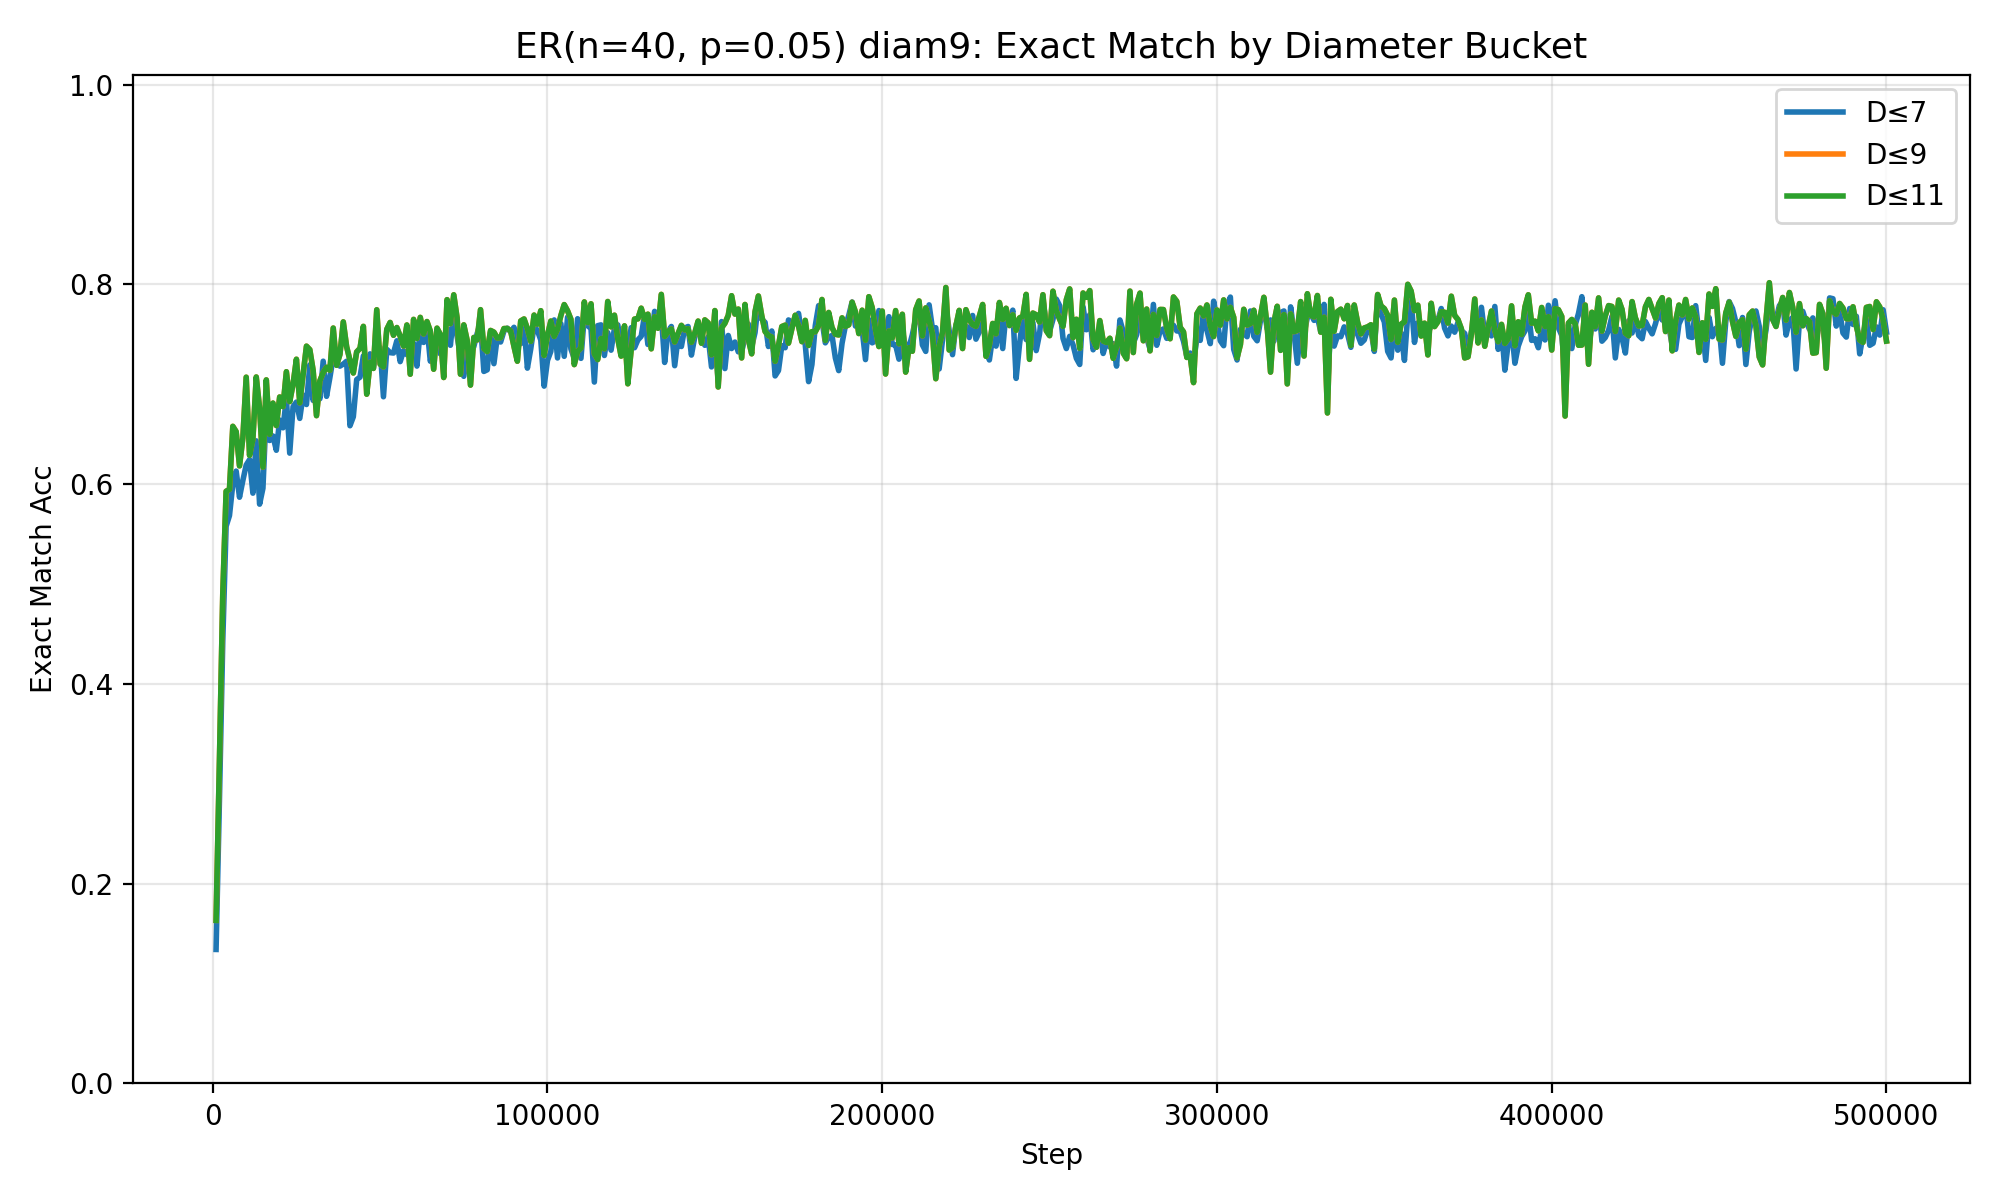
\includegraphics[width=\textwidth]{runs/retrain_er_n40_485351/n40_p005_diam9/er_n40_diam9_per_diam_bucket.png}
        \caption{Exact match per test-graph diameter bucket.}
    \end{subfigure}

    \vspace{1em}

    \begin{subfigure}[t]{0.6\textwidth}
        \centering
        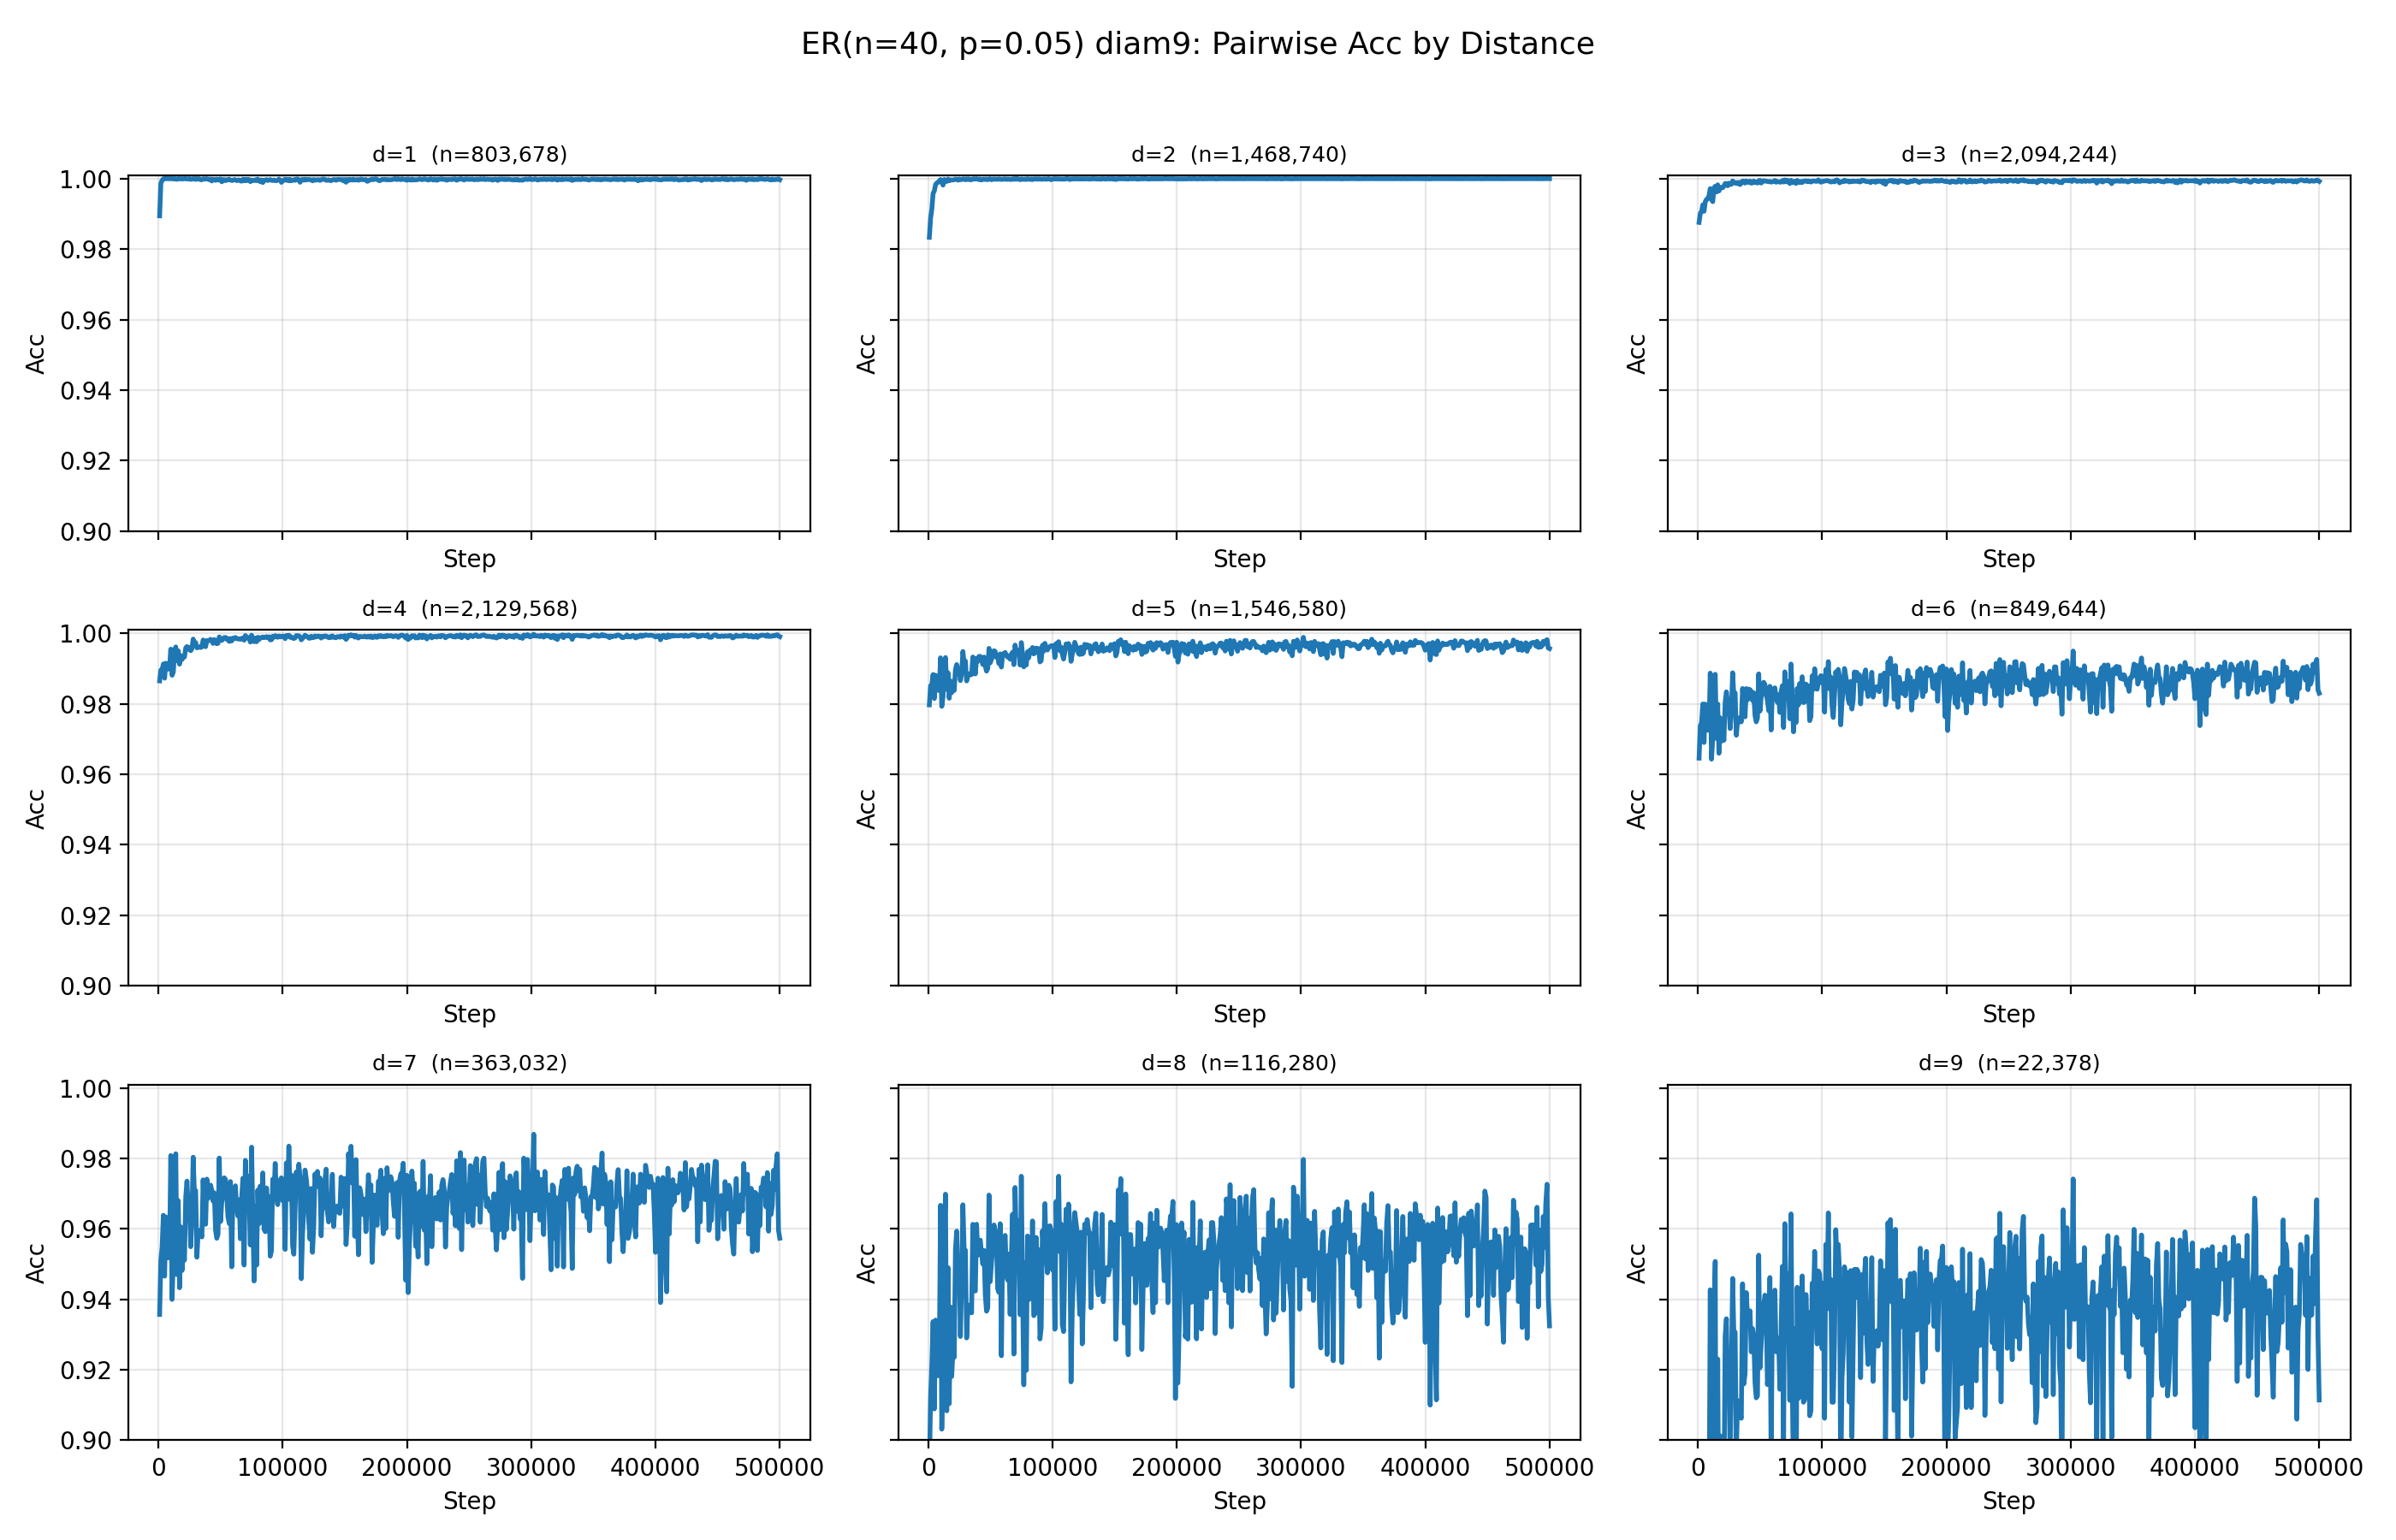
\includegraphics[width=\textwidth]{runs/retrain_er_n40_485351/n40_p005_diam9/er_n40_diam9_per_dist_sm.png}
        \caption{Pairwise accuracy by shortest-path distance. The number above each panel is the count of test pairs at that distance.}
    \end{subfigure}

    \caption{$D \le 9$, in distribution.}
\end{figure}

\begin{figure}[H]
    \centering
    \begin{subfigure}[t]{0.66\textwidth}
        \centering
        
\includegraphics[width=\textwidth]{runs/ood_cross_experiment/ood_n40_diam9_per_distance_bars.png}
        \caption{Per-distance pairwise accuracy on the three OOD sets.}
    \end{subfigure}
    \hfill
    \begin{subfigure}[t]{0.32\textwidth}
        \centering
        
\includegraphics[width=\textwidth]{runs/ood_cross_experiment/ood_n40_diam9_per_diam_bucket.png}
        \caption{Exact match on unfiltered ER by diameter bucket.}
    \end{subfigure}
    \caption{$D \le 9$, OOD.}
\end{figure}

\subsubsection{$D \le 7$}

\begin{figure}[H]
    \centering
    \begin{subfigure}[t]{0.32\textwidth}
        \centering
        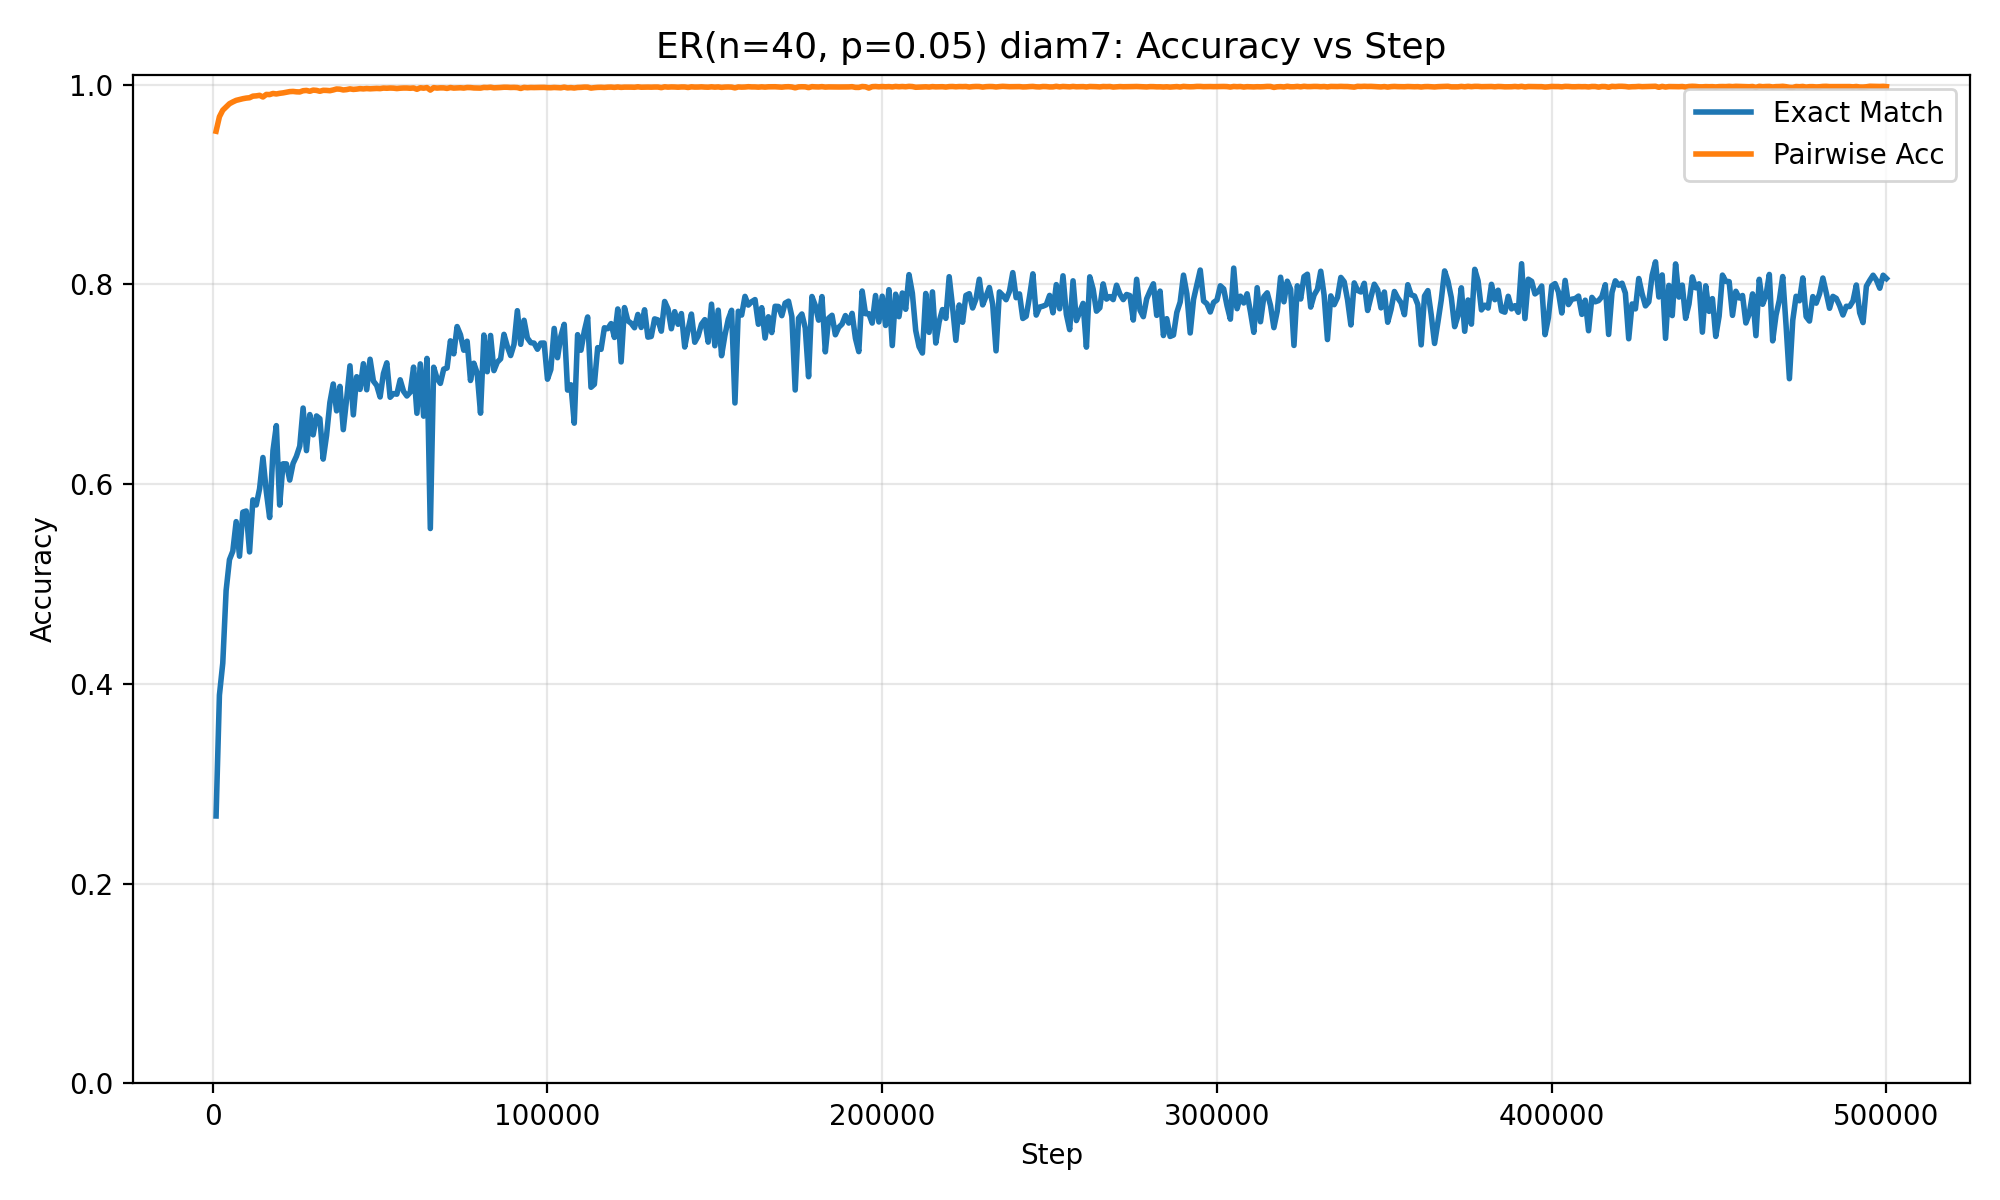
\includegraphics[width=\textwidth]{runs/retrain_er_n40_485353/n40_p005_diam7/er_n40_diam7_accuracy.png}
        \caption{Exact match and pairwise accuracy.}
    \end{subfigure}
    \hfill
    \begin{subfigure}[t]{0.32\textwidth}
        \centering
        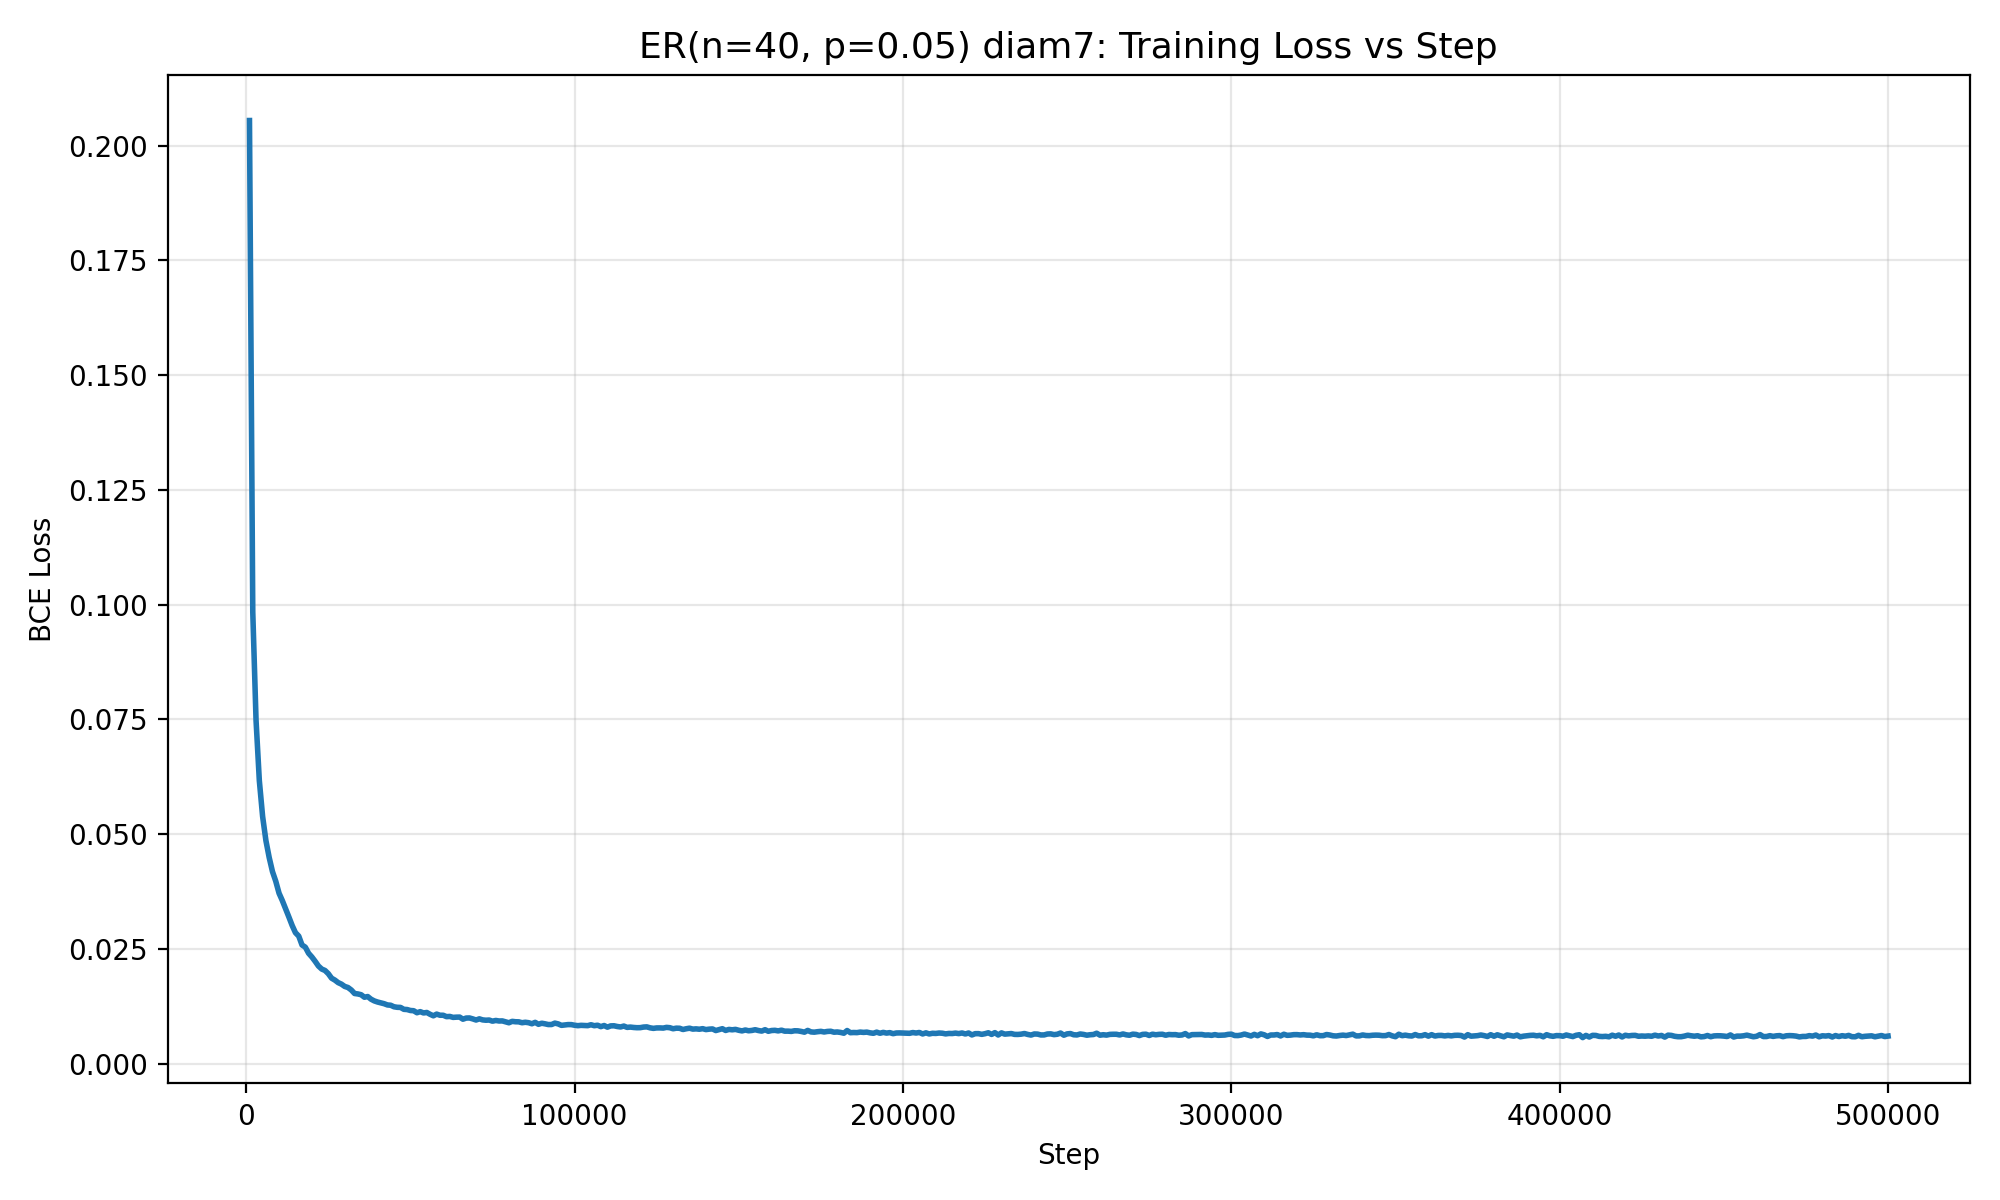
\includegraphics[width=\textwidth]{runs/retrain_er_n40_485353/n40_p005_diam7/er_n40_diam7_loss.png}
        \caption{Training loss.}
    \end{subfigure}
    \hfill
    \begin{subfigure}[t]{0.32\textwidth}
        \centering
        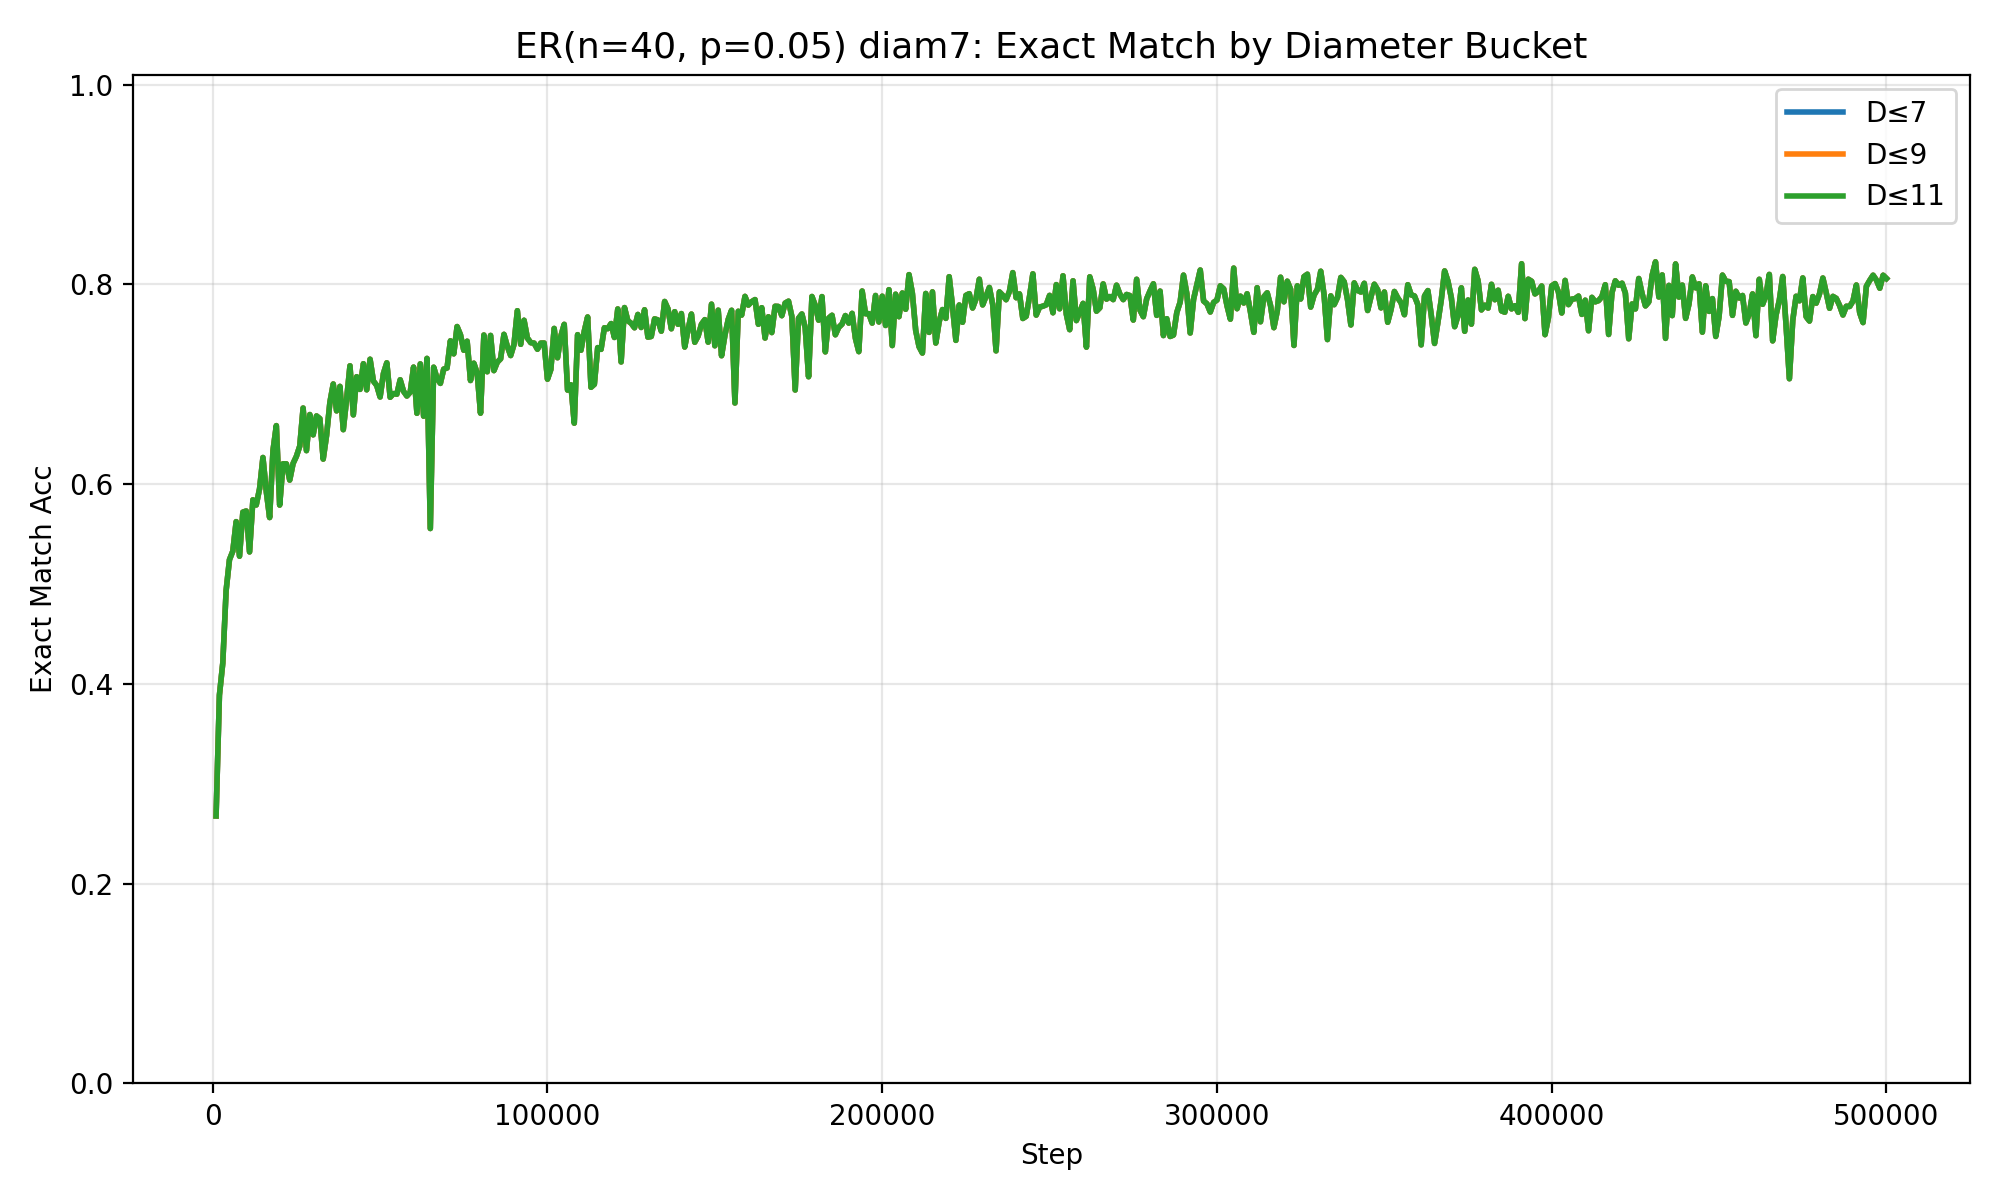
\includegraphics[width=\textwidth]{runs/retrain_er_n40_485353/n40_p005_diam7/er_n40_diam7_per_diam_bucket.png}
        \caption{Exact match per test-graph diameter bucket.}
    \end{subfigure}

    \vspace{1em}

    \begin{subfigure}[t]{0.6\textwidth}
        \centering
        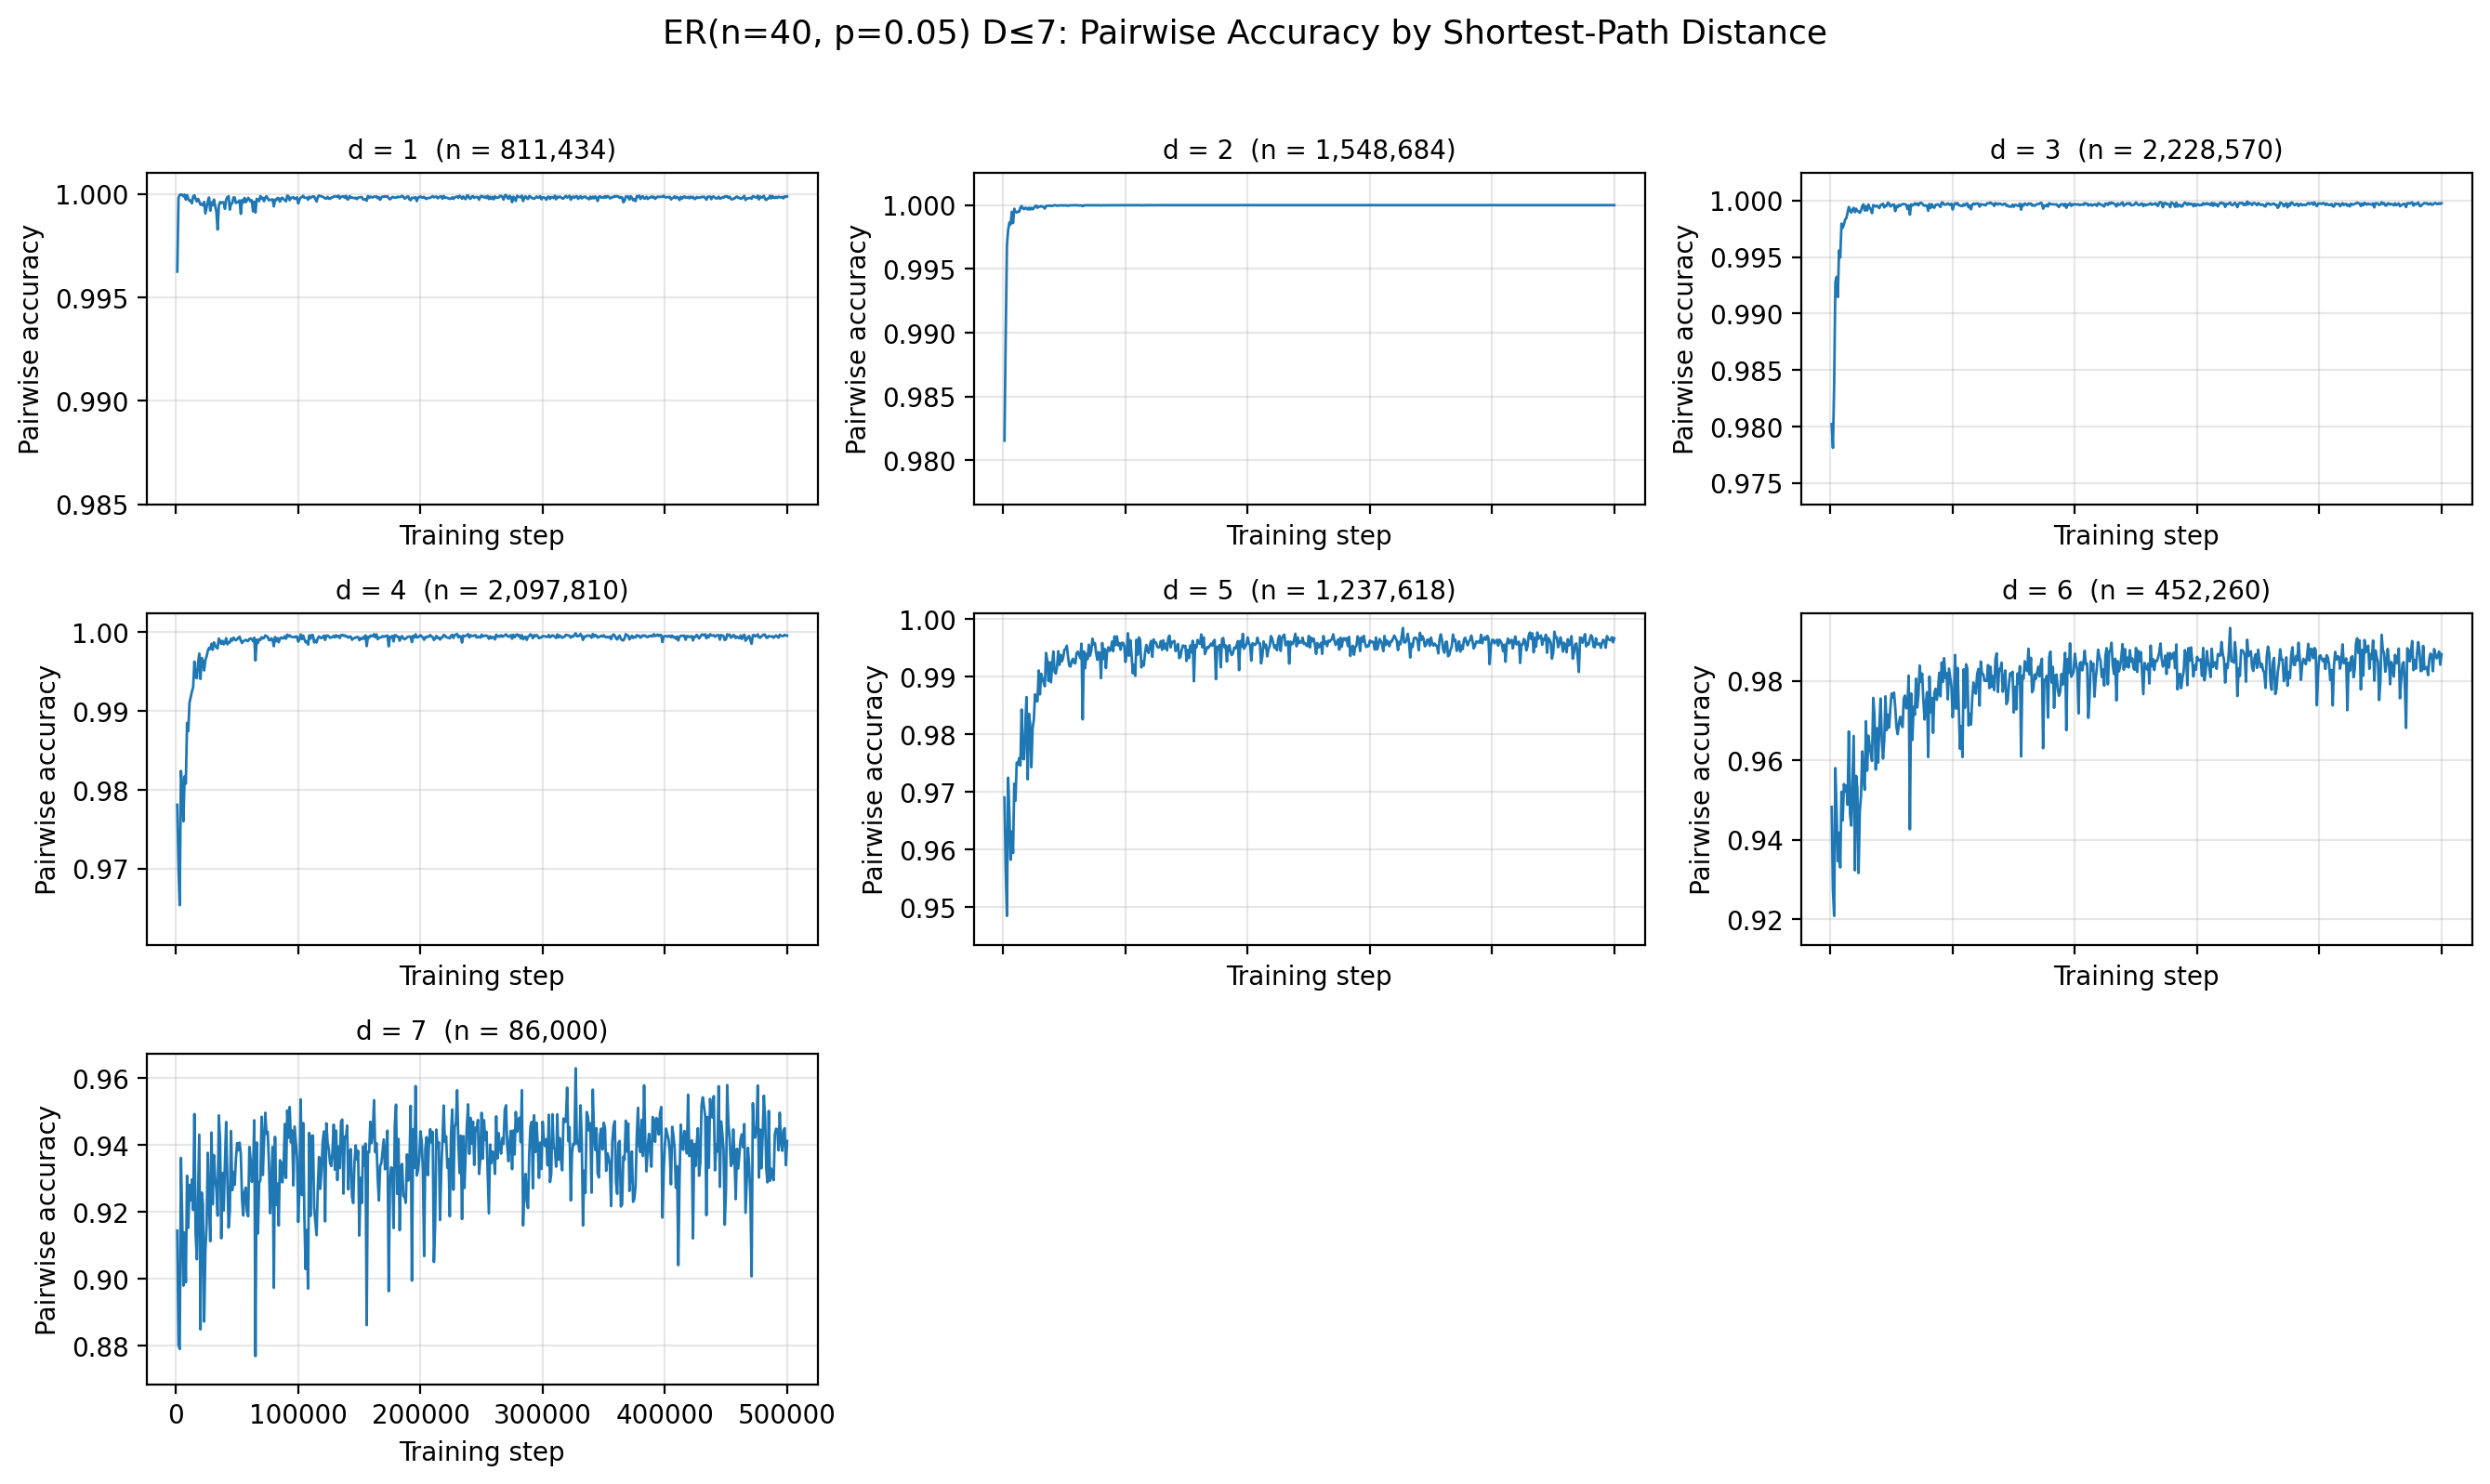
\includegraphics[width=\textwidth]{runs/retrain_er_n40_485353/n40_p005_diam7/er_n40_diam7_per_dist_sm.png}
        \caption{Pairwise accuracy by shortest-path distance. The number above each panel is the count of test pairs at that distance.}
    \end{subfigure}

    \caption{$D \le 7$, in distribution.}
\end{figure}

\begin{figure}[H]
    \centering
    \begin{subfigure}[t]{0.66\textwidth}
        \centering
        
\includegraphics[width=\textwidth]{runs/ood_cross_experiment/ood_n40_diam7_per_distance_bars.png}
        \caption{Per-distance pairwise accuracy on the three OOD sets.}
    \end{subfigure}
    \hfill
    \begin{subfigure}[t]{0.32\textwidth}
        \centering
        
\includegraphics[width=\textwidth]{runs/ood_cross_experiment/ood_n40_diam7_per_diam_bucket.png}
        \caption{Exact match on unfiltered ER by diameter bucket.}
    \end{subfigure}
    \caption{$D \le 7$, OOD.}
\end{figure}

\subsection{Comments on Chapter~\ref{sec:ch2}}

The four diameter-controlled small-model runs reach essentially the same
in-distribution exact-match accuracy ($\approx 0.80$) but converge at
very different speeds. The diameter filter helps the model
\emph{learn faster}, but the final achievable accuracy does not depend on
the filter in this setup. The fact that all four runs converge to the
same accuracy is the main reason we then re-ran the same protocol with a
larger model in Chapter~\ref{sec:ch3}: if the bottleneck is model size
rather than training distribution, the data lever effect should become
more visible once the model is large enough to actually fit the easier
filtered distributions.

On the OOD side, the picture is already mostly negative for the data
lever in the standard-transformer setting. The unfiltered model is the
most robust on 2-chains transfer, no model gets any 2-cliques graph
exactly right at $n_{\text{active}} > 14$, and on the unfiltered-ER
per-bucket evaluation the unfiltered model is competitive with each
diameter specialist on the specialist's bucket and is strictly better on
the $D > 11$ bucket. The $D \le 9$ configuration that the disentangled
theory predicts as the empirical optimum for $L = 2$ is, by every metric
we measure, not the best of the four.

\vspace{2em}

\section{Chapter 3 --- Diameter-controlled training on ER$(n = 40)$ (large model)}
\label{sec:ch3}

\subsection{Motivation and setup}

The Chapter~\ref{sec:ch2} experiments left a clean motivating question.
The four small-model runs converge at very different speeds but settle at
the same in-distribution exact-match accuracy of about $0.80$, which is
consistent with a model-size rather than data-distribution bottleneck.
Two follow-up actions are therefore natural: increase the model capacity
to lift this ceiling, and re-run the diameter-controlled comparison in
the regime where every run reaches near-perfect in-distribution accuracy,
so that we can read OOD performance without the in-distribution number
acting as a confound.

We use the large configuration of Section~\ref{sec:model}: $L = 2$
attention layers, $d_{\mathrm{model}} = 512$, $d_{\mathrm{ff}} = 2048$,
$4$ attention heads, normalised-ReLU attention, bf16 mixed precision,
online streaming of training graphs (each training graph is freshly
sampled by rejection sampling at each step, so the model never sees the
same graph twice), batch size $1{,}000$ and a training budget of
$1{,}000{,}000$ optimisation steps. We additionally include a 4-phase
\emph{curriculum} run that starts on $D \le 7$, advances to $D \le 9$,
$D \le 10$ and finally $D \le 11$, with each phase boundary triggered by
the smoothed training loss falling below a pre-set threshold; the
combined budget is again $1{,}000{,}000$ steps. All five runs share the
same optimiser, model size, and OOD evaluation protocol.

\subsection{Cross-experiment view: convergence and final accuracy}

Table~\ref{tab:big-summary} reports best in-distribution exact match,
convergence steps to the $0.99$ exact-match milestone, and a few finer
milestones for the five large-model runs.

\begin{table}[H]
\centering
\begin{tabular}{lcccc}
\toprule
Experiment & Best exact match & step @ EM $\ge 0.99$ & step @ EM $\ge 0.999$ & step @ EM $\ge 0.9999$ \\
\midrule
Unfiltered   & 0.9997 & $180{,}000$ & $570{,}000$ & --- \\
$D \le 11$   & 0.9998 & $120{,}000$ & $535{,}000$ & --- \\
Curriculum   & 0.9998 & $110{,}000$ & $485{,}000$ & --- \\
$D \le 9$    & 1.0000 & $\phantom{0}85{,}000$ & $330{,}000$ & $500{,}000$ \\
$D \le 7$    & 1.0000 & $\phantom{0}\textbf{10{,}000}$ & $\phantom{0}\textbf{85{,}000}$ & $\textbf{170{,}000}$ \\
\bottomrule
\end{tabular}
\caption{Convergence summary for the five large-model runs. All runs use
online streaming and $1{,}000{,}000$ optimisation steps.
``Step @ EM $\ge x$'' is the first evaluation step at which exact-match
accuracy on the held-out test set reaches the threshold $x$. A dash
indicates that the threshold was not reached during training.}
\label{tab:big-summary}
\end{table}

The convergence ordering is the same one already observed for the small
model in Chapter~\ref{sec:ch2}: convergence speed is monotone in the
diameter filter, with $D \le 7$ the fastest and unfiltered the slowest.
Two differences with respect to Chapter~\ref{sec:ch2} are worth noting:
\begin{itemize}
    \item Every large-model run reaches $\ge 0.9995$ in-distribution
          exact match; the $0.80$ ceiling of the small model is gone.
    \item The curriculum run lands essentially on the $D \le 11$ run.
          A glance at the run's phase log makes this obvious: the loss
          thresholds for phases $1$--$3$ are met within $30{,}000$ steps
          total, so the curriculum spends about $970{,}000$ of its
          $1{,}000{,}000$ steps in the final $D \le 11$ phase. The
          curriculum as configured is therefore close to ``$D \le 11$
          with a short $D \le 7$ warm-up''.
\end{itemize}

\subsection{Cross-experiment view: out-of-distribution}
\label{sec:ch3-cross-ood}

We re-evaluate each of the five large-model runs on:
\begin{itemize}
    \item \textbf{2-chains} with $n_{\text{active}} \in \{14, 16, \ldots, 40\}$,
          padded to $40 \times 40$;
    \item \textbf{2-cliques} with the same protocol;
    \item \textbf{Unfiltered ER}$(40, 0.05)$, with the per-graph-diameter
          breakdown.
\end{itemize}
Each test set contains $10{,}000$ graphs.

\subsubsection*{2-chains: exact-match cliff by $n_{\text{active}}$}

\begin{table}[H]
\centering
\begin{tabular}{lccccc}
\toprule
$n_{\text{active}}$ & Unfiltered & $D \le 11$ & $D \le 9$ & $D \le 7$ & Curriculum \\
\midrule
$14, 16$  & 1.00 & 1.00 & 1.00 & 1.00 & 1.00 \\
$18, 20$  & 1.00 & 1.00 & 1.00 & \textbf{0.00} & 1.00 \\
$\ge 22$  & 0.00 & 0.00 & 0.00 & 0.00 & 0.00 \\
\bottomrule
\end{tabular}
\caption{Exact-match accuracy on the 2-chains OOD set as a function of
$n_{\text{active}}$, grouped over rows with identical behaviour. Each
$n_{\text{active}}$ bin contains $\approx 700$ graphs.}
\label{tab:big-chains-byn}
\end{table}

Four of the five models (unfiltered, $D \le 11$, $D \le 9$, curriculum)
exhibit the same step function: exact match $1.0$ up to
$n_{\text{active}} = 20$, then $0.0$ from $n_{\text{active}} = 22$
onward. The $D \le 7$ model loses two additional bins
($n_{\text{active}} = 18, 20$). In other words, on 2-chains the data
lever does not help in the large-model regime either: the unfiltered
model and the three filtered models are indistinguishable from each
other, with the only effect of the tightest filter ($D \le 7$) being to
move the cliff earlier.

\subsubsection*{2-cliques}

All five large-model runs reach exact match $0$ at every
$n_{\text{active}}$ on the 2-cliques OOD set. The pairwise accuracy is in
$0.74$--$0.77$ across runs, and the per-distance breakdown shows a small
but consistent ordering: the $D \le 7$ and $D \le 9$ models recognise
the within-clique $d = 1$ pairs better than the unfiltered model
($0.42$ and $0.36$ respectively, versus $0.08$ for unfiltered and
$0.0$ for $D \le 11$), at the cost of slightly worse accuracy on the
``disconnected'' across-clique pairs. The net effect on exact match is
zero. We highlight this in passing because it is the only setting in
which a filtered run has a sub-metric that exceeds the unfiltered model;
the overall picture remains that the data lever does not produce a
2-cliques generalisation for the standard transformer at $n = 40$.

\subsubsection*{Unfiltered ER, by graph diameter}

\begin{table}[H]
\centering
\begin{tabular}{lccccc}
\toprule
Model       & $D \le 7$ & $D \le 9$ & $D \le 11$ & $D > 11$ & overall \\
\midrule
Unfiltered  & 1.000 & 0.9996 & 0.9991 & \textbf{0.9986} & \textbf{0.9990} \\
$D \le 11$  & 1.000 & 0.9996 & 0.9989 & 0.9807 & 0.9963 \\
Curriculum  & 1.000 & 0.9996 & 0.9991 & 0.9704 & 0.9949 \\
$D \le 9$   & 1.000 & \textbf{1.0000} & 0.9883 & 0.5882 & 0.9302 \\
$D \le 7$   & \textbf{1.000} & 0.9277 & 0.7547 & 0.0324 & 0.6498 \\
\bottomrule
\end{tabular}
\caption{Exact-match accuracy on a fixed test set of $10{,}000$
unfiltered ER$(40, 0.05)$ graphs, broken down by the test-graph
diameter, for the five large-model runs (number of graphs per bucket:
$1{,}329$, $5{,}574$, $8{,}548$, $1{,}452$). Bold entries mark the best
model in each column.}
\label{tab:ood-er-buckets-big}
\end{table}

With every large-model run essentially perfect inside its training
diameter budget, the table is a clean read of the data lever's actual
effect. The unfiltered model is strictly best (or tied) on every
diameter bucket and is overall the most accurate of the five. The
filtered models are perfect on their training bucket and degrade
monotonically on buckets above the cut-off, with the degradation
becoming sharper the tighter the filter. The curriculum sits between
$D \le 11$ and unfiltered.

\subsection{Per-experiment figures (large model)}

The following subsections collect the in-distribution training curves
and the per-experiment OOD plots used in the cross-experiment view
above.

\subsubsection{Unfiltered}

\begin{figure}[H]
    \centering
    \begin{subfigure}[t]{0.32\textwidth}
        \centering
        
\includegraphics[width=\textwidth]{runs/retrain_er_n40_big_495903/n40_p005_unfiltered_big/er_n40_unfiltered_big_accuracy.png}
        \caption{Exact match and pairwise accuracy.}
    \end{subfigure}
    \hfill
    \begin{subfigure}[t]{0.32\textwidth}
        \centering
        
\includegraphics[width=\textwidth]{runs/retrain_er_n40_big_495903/n40_p005_unfiltered_big/er_n40_unfiltered_big_loss.png}
        \caption{Training loss.}
    \end{subfigure}
    \hfill
    \begin{subfigure}[t]{0.32\textwidth}
        \centering
        
\includegraphics[width=\textwidth]{runs/retrain_er_n40_big_495903/n40_p005_unfiltered_big/er_n40_unfiltered_big_per_diam_bucket.png}
        \caption{Exact match per test-graph diameter bucket.}
    \end{subfigure}

    \vspace{1em}

    \begin{subfigure}[t]{0.6\textwidth}
        \centering
        
\includegraphics[width=\textwidth]{runs/retrain_er_n40_big_495903/n40_p005_unfiltered_big/er_n40_unfiltered_big_per_dist_sm.png}
        \caption{Pairwise accuracy by shortest-path distance. The number above each panel is the count of test pairs at that distance.}
    \end{subfigure}

    \caption{Large model, Unfiltered, in distribution.}
\end{figure}

\begin{figure}[H]
    \centering
    \begin{subfigure}[t]{0.85\textwidth}
        \centering
        
\includegraphics[width=\textwidth]{runs/ood_eval_n40_big_495904/er_n40_big_unfiltered_to_structured/per_distance_bars.png}
        \caption{Per-distance pairwise accuracy on the three OOD sets.}
    \end{subfigure}

    \vspace{1em}

    \begin{subfigure}[t]{0.49\textwidth}
        \centering
        
\includegraphics[width=\textwidth]{runs/ood_eval_n40_big_495904/er_n40_big_unfiltered_to_structured/per_diam_bucket_ood.png}
        \caption{Exact match on unfiltered ER by diameter bucket.}
    \end{subfigure}
    \hfill
    \begin{subfigure}[t]{0.49\textwidth}
        \centering
        
\includegraphics[width=\textwidth]{runs/ood_eval_n40_big_495904/er_n40_big_unfiltered_to_structured/per_n_active.png}
        \caption{Exact match on 2-chains and 2-cliques as a function of
        $n_{\text{active}}$.}
    \end{subfigure}

    \caption{Large model, Unfiltered, OOD.}
\end{figure}

\subsubsection{$D \le 11$}

\begin{figure}[H]
    \centering
    \begin{subfigure}[t]{0.32\textwidth}
        \centering
        
\includegraphics[width=\textwidth]{runs/retrain_er_n40_big_494467/n40_p005_diam11_big/er_n40_diam11_big_accuracy.png}
        \caption{Exact match and pairwise accuracy.}
    \end{subfigure}
    \hfill
    \begin{subfigure}[t]{0.32\textwidth}
        \centering
        
\includegraphics[width=\textwidth]{runs/retrain_er_n40_big_494467/n40_p005_diam11_big/er_n40_diam11_big_loss.png}
        \caption{Training loss.}
    \end{subfigure}
    \hfill
    \begin{subfigure}[t]{0.32\textwidth}
        \centering
        
\includegraphics[width=\textwidth]{runs/retrain_er_n40_big_494467/n40_p005_diam11_big/er_n40_diam11_big_per_diam_bucket.png}
        \caption{Exact match per test-graph diameter bucket.}
    \end{subfigure}

    \vspace{1em}

    \begin{subfigure}[t]{0.6\textwidth}
        \centering
        
\includegraphics[width=\textwidth]{runs/retrain_er_n40_big_494467/n40_p005_diam11_big/er_n40_diam11_big_per_dist_sm.png}
        \caption{Pairwise accuracy by shortest-path distance. The number above each panel is the count of test pairs at that distance.}
    \end{subfigure}

    \caption{Large model, $D \le 11$, in distribution.}
\end{figure}

\begin{figure}[H]
    \centering
    \begin{subfigure}[t]{0.85\textwidth}
        \centering
        
\includegraphics[width=\textwidth]{runs/ood_eval_n40_big_495904/er_n40_big_diam11_to_structured/per_distance_bars.png}
        \caption{Per-distance pairwise accuracy on the three OOD sets.}
    \end{subfigure}

    \vspace{1em}

    \begin{subfigure}[t]{0.49\textwidth}
        \centering
        
\includegraphics[width=\textwidth]{runs/ood_eval_n40_big_495904/er_n40_big_diam11_to_structured/per_diam_bucket_ood.png}
        \caption{Exact match on unfiltered ER by diameter bucket.}
    \end{subfigure}
    \hfill
    \begin{subfigure}[t]{0.49\textwidth}
        \centering
        
\includegraphics[width=\textwidth]{runs/ood_eval_n40_big_495904/er_n40_big_diam11_to_structured/per_n_active.png}
        \caption{Exact match on 2-chains and 2-cliques as a function of
        $n_{\text{active}}$.}
    \end{subfigure}

    \caption{Large model, $D \le 11$, OOD.}
\end{figure}

\subsubsection{$D \le 9$}

\begin{figure}[H]
    \centering
    \begin{subfigure}[t]{0.32\textwidth}
        \centering
        
\includegraphics[width=\textwidth]{runs/retrain_er_n40_big_495198/n40_p005_diam9_big/er_n40_diam9_big_accuracy.png}
        \caption{Exact match and pairwise accuracy.}
    \end{subfigure}
    \hfill
    \begin{subfigure}[t]{0.32\textwidth}
        \centering
        
\includegraphics[width=\textwidth]{runs/retrain_er_n40_big_495198/n40_p005_diam9_big/er_n40_diam9_big_loss.png}
        \caption{Training loss.}
    \end{subfigure}
    \hfill
    \begin{subfigure}[t]{0.32\textwidth}
        \centering
        
\includegraphics[width=\textwidth]{runs/retrain_er_n40_big_495198/n40_p005_diam9_big/er_n40_diam9_big_per_diam_bucket.png}
        \caption{Exact match per test-graph diameter bucket.}
    \end{subfigure}

    \vspace{1em}

    \begin{subfigure}[t]{0.6\textwidth}
        \centering
        
\includegraphics[width=\textwidth]{runs/retrain_er_n40_big_495198/n40_p005_diam9_big/er_n40_diam9_big_per_dist_sm.png}
        \caption{Pairwise accuracy by shortest-path distance. The number above each panel is the count of test pairs at that distance.}
    \end{subfigure}

    \caption{Large model, $D \le 9$, in distribution.}
\end{figure}

\begin{figure}[H]
    \centering
    \begin{subfigure}[t]{0.85\textwidth}
        \centering
        
\includegraphics[width=\textwidth]{runs/ood_eval_n40_big_495904/er_n40_big_diam9_to_structured/per_distance_bars.png}
        \caption{Per-distance pairwise accuracy on the three OOD sets.}
    \end{subfigure}

    \vspace{1em}

    \begin{subfigure}[t]{0.49\textwidth}
        \centering
        
\includegraphics[width=\textwidth]{runs/ood_eval_n40_big_495904/er_n40_big_diam9_to_structured/per_diam_bucket_ood.png}
        \caption{Exact match on unfiltered ER by diameter bucket.}
    \end{subfigure}
    \hfill
    \begin{subfigure}[t]{0.49\textwidth}
        \centering
        
\includegraphics[width=\textwidth]{runs/ood_eval_n40_big_495904/er_n40_big_diam9_to_structured/per_n_active.png}
        \caption{Exact match on 2-chains and 2-cliques as a function of
        $n_{\text{active}}$.}
    \end{subfigure}

    \caption{Large model, $D \le 9$, OOD.}
\end{figure}

\subsubsection{$D \le 7$}

\begin{figure}[H]
    \centering
    \begin{subfigure}[t]{0.32\textwidth}
        \centering
        
\includegraphics[width=\textwidth]{runs/retrain_er_n40_big_495199/n40_p005_diam7_big/er_n40_diam7_big_accuracy.png}
        \caption{Exact match and pairwise accuracy.}
    \end{subfigure}
    \hfill
    \begin{subfigure}[t]{0.32\textwidth}
        \centering
        
\includegraphics[width=\textwidth]{runs/retrain_er_n40_big_495199/n40_p005_diam7_big/er_n40_diam7_big_loss.png}
        \caption{Training loss.}
    \end{subfigure}
    \hfill
    \begin{subfigure}[t]{0.32\textwidth}
        \centering
        
\includegraphics[width=\textwidth]{runs/retrain_er_n40_big_495199/n40_p005_diam7_big/er_n40_diam7_big_per_diam_bucket.png}
        \caption{Exact match per test-graph diameter bucket.}
    \end{subfigure}

    \vspace{1em}

    \begin{subfigure}[t]{0.6\textwidth}
        \centering
        
\includegraphics[width=\textwidth]{runs/retrain_er_n40_big_495199/n40_p005_diam7_big/er_n40_diam7_big_per_dist_sm.png}
        \caption{Pairwise accuracy by shortest-path distance. The number above each panel is the count of test pairs at that distance.}
    \end{subfigure}

    \caption{Large model, $D \le 7$, in distribution.}
\end{figure}

\begin{figure}[H]
    \centering
    \begin{subfigure}[t]{0.85\textwidth}
        \centering
        
\includegraphics[width=\textwidth]{runs/ood_eval_n40_big_495904/er_n40_big_diam7_to_structured/per_distance_bars.png}
        \caption{Per-distance pairwise accuracy on the three OOD sets.}
    \end{subfigure}

    \vspace{1em}

    \begin{subfigure}[t]{0.49\textwidth}
        \centering
        
\includegraphics[width=\textwidth]{runs/ood_eval_n40_big_495904/er_n40_big_diam7_to_structured/per_diam_bucket_ood.png}
        \caption{Exact match on unfiltered ER by diameter bucket.}
    \end{subfigure}
    \hfill
    \begin{subfigure}[t]{0.49\textwidth}
        \centering
        
\includegraphics[width=\textwidth]{runs/ood_eval_n40_big_495904/er_n40_big_diam7_to_structured/per_n_active.png}
        \caption{Exact match on 2-chains and 2-cliques as a function of
        $n_{\text{active}}$.}
    \end{subfigure}

    \caption{Large model, $D \le 7$, OOD.}
\end{figure}

\subsubsection{Curriculum}

\begin{figure}[H]
    \centering
    \begin{subfigure}[t]{0.32\textwidth}
        \centering
        
\includegraphics[width=\textwidth]{runs/curriculum_er_n40_big_494470/n40_p005_curriculum_big/curriculum_er_n40_big_accuracy.png}
        \caption{Exact match and pairwise accuracy.}
    \end{subfigure}
    \hfill
    \begin{subfigure}[t]{0.32\textwidth}
        \centering
        
\includegraphics[width=\textwidth]{runs/curriculum_er_n40_big_494470/n40_p005_curriculum_big/curriculum_er_n40_big_loss.png}
        \caption{Training loss.}
    \end{subfigure}
    \hfill
    \begin{subfigure}[t]{0.32\textwidth}
        \centering
        
\includegraphics[width=\textwidth]{runs/curriculum_er_n40_big_494470/n40_p005_curriculum_big/curriculum_er_n40_big_per_diam_bucket.png}
        \caption{Exact match per test-graph diameter bucket.}
    \end{subfigure}

    \vspace{1em}

    \begin{subfigure}[t]{0.6\textwidth}
        \centering
        
\includegraphics[width=\textwidth]{runs/curriculum_er_n40_big_494470/n40_p005_curriculum_big/curriculum_er_n40_big_per_dist_sm.png}
        \caption{Pairwise accuracy by shortest-path distance. The number above each panel is the count of test pairs at that distance.}
    \end{subfigure}

    \caption{Large model, Curriculum, in distribution.}
\end{figure}

\begin{table}[H]
\centering
\begin{tabular}{lc}
\toprule
Phase (filter) & Start step \\
\midrule
1 ($D \le 7$)  & $0$ \\
2 ($D \le 9$)  & $20{,}000$ \\
3 ($D \le 10$) & $25{,}000$ \\
4 ($D \le 11$) & $30{,}000$ \\
\bottomrule
\end{tabular}
\caption{Curriculum phase transitions. Phases $1$--$3$ are advanced as
soon as the smoothed training loss falls below a preset threshold; phase
$4$ runs to the end of the $1{,}000{,}000$-step budget. Phases $1$--$3$
close within the first $30{,}000$ steps, so the remaining
$\sim 970{,}000$ steps are spent on $D \le 11$.}
\label{tab:curriculum-phases}
\end{table}

\begin{figure}[H]
    \centering
    \begin{subfigure}[t]{0.85\textwidth}
        \centering
        
\includegraphics[width=\textwidth]{runs/ood_eval_curriculum_big_494472/er_n40_big_curriculum_to_structured/per_distance_bars.png}
        \caption{Per-distance pairwise accuracy on the three OOD sets.}
    \end{subfigure}

    \vspace{1em}

    \begin{subfigure}[t]{0.49\textwidth}
        \centering
        
\includegraphics[width=\textwidth]{runs/ood_eval_curriculum_big_494472/er_n40_big_curriculum_to_structured/per_diam_bucket_ood.png}
        \caption{Exact match on unfiltered ER by diameter bucket.}
    \end{subfigure}
    \hfill
    \begin{subfigure}[t]{0.49\textwidth}
        \centering
        
\includegraphics[width=\textwidth]{runs/ood_eval_curriculum_big_494472/er_n40_big_curriculum_to_structured/per_n_active.png}
        \caption{Exact match on 2-chains and 2-cliques as a function of
        $n_{\text{active}}$.}
    \end{subfigure}

    \caption{Large model, Curriculum, OOD.}
\end{figure}

\subsection{Comments on Chapter~\ref{sec:ch3}}

Two observations summarise the large-model results.

First, raising the model from $\sim 72$k to $\sim 6.3$M parameters
lifts the $0.80$ in-distribution ceiling of Chapter~\ref{sec:ch2}. All
five large-model runs reach $\ge 0.9995$ in-distribution exact match,
and the convergence ordering across diameter filters is the same we
already saw in the small-model regime: tighter filter, faster
convergence.

Second, none of the OOD tests we ran show a benefit of the diameter
filter in the large-model regime either. The unfiltered model is strictly
best (or tied) on every bucket of the per-diameter unfiltered-ER
evaluation, the diameter-restricted models exhibit a sharp accuracy
cliff just above their cut-off, the 2-chains exact-match cliff at
$n_{\text{active}} = 22$ is the same for unfiltered, $D \le 11$,
$D \le 9$ and curriculum (and is earlier for $D \le 7$), and all five
runs reach exact match $0$ on 2-cliques. The only sub-metric on which a
filtered run exceeds the unfiltered model is within-clique $d = 1$
pairwise accuracy ($D \le 7$ at $0.42$, $D \le 9$ at $0.36$, versus
$0.08$ for unfiltered), which does not translate into any improvement
at the graph level. We do not draw a strong conclusion from this single
sub-metric.

Combined with Chapter~\ref{sec:ch2}, the empirical picture is consistent
between the two model scales: in our standard-transformer setup the data
lever helps the model learn faster but does not produce the OOD benefits
predicted by the disentangled-transformer analysis. Whether this
discrepancy is due to the architectural simplification between the
disentangled and standard transformers, to the difference in scale
($n = 40$ here versus $n = 20$ in the original experiments), or to some
combination of both, is not something our experiments can directly settle.

\end{document}
